\chapter{三角比与角边关系}

人们为了要确定空间各点之间的相互位置,就得做一番
测量,测量是几何学的起源,也是几何学最直接的实践。

测量学的最基本原理,就是相似形的性质及三角形的边
角关系。例如,我们在第三章末用相似形性质测量两点间的,
距离,物体的高度、测绘具有多边形形状的地段的平面图
等。我们知道,在两个直角三角形中,只要有一个锐角对应
相等,它们就相似了,这就是说,一个直角三角形的各边之。
间的比是被它的一个锐角的大小所决定,例如在图6.1中,
一些含有$30^{\circ}$角的直角三角形,$30^{\circ}$角所对的直角边与斜边的
比都是1:2.

\begin{figure}[htp]
    \centering
\begin{tikzpicture}
\begin{scope}
\tkzDefPoint(30:2){B_1}
\tkzDefPoints{0/0/A_1, 1.732/0/C_1}
\tkzDrawPolygon(A_1,B_1,C_1)
\tkzMarkAngle[mark=none, size=.5](C_1,A_1,B_1)
\tkzLabelPoints[right](C_1,B_1)
\tkzLabelPoints[left](A_1)
\tkzMarkRightAngle(B_1,C_1,A_1)
\end{scope}
\begin{scope}[xshift=3.5cm]
    \tkzDefPoint(30:3){B_2}
    \tkzDefPoints{0/0/A_2, 2.6/0/C_2}
    \tkzDrawPolygon(A_2,B_2,C_2)
    \tkzMarkAngle[mark=none, size=.5](C_2,A_2,B_2)
    \tkzLabelPoints[right](C_2,B_2)
    \tkzLabelPoints[left](A_2)
    \tkzMarkRightAngle(B_2,C_2,A_2)
\end{scope}
\begin{scope}[xshift=11cm]
    \tkzDefPoint(150:4){B_3}
    \tkzDefPoints{0/0/A_3, -3.464/0/C_3}
    \tkzDrawPolygon(A_3,B_3,C_3)
    \tkzMarkAngle[mark=none, size=.6](B_3,A_3,C_3)
    \tkzLabelPoints[below](C_3,A_3)
    \tkzLabelPoints[left](B_3) 
    \tkzMarkRightAngle(A_3,C_3,B_3)
\end{scope}

\end{tikzpicture}
    \caption{}
\end{figure}

这一章,我们首先向同学介绍的就是直角三角形中,边
与边的比与它所含锐角之间的关系。这些边与边的比值叫做
\textbf{锐角三角比},它们是进行测量计算时的常用数据,也是从数
量方面研究几何学的基本工具。

\section{锐角三角比}

\subsection{定义}

\begin{figure}[htp]\centering
    \begin{minipage}[t]{0.48\textwidth}
    \centering
\begin{tikzpicture}[>=latex, scale=.8]
\draw(30:6)node[right]{$Y$}--(0,0)node[left]{$A$}--(5.5,0)node[right]{$X$};
\draw(30:5)node[above]{$B$}--node[right]{$a$}+(0,-2.5)node[below]{$C$};
\node at (1.25*1.732,0)[below]{$b$};
\node at (30:2.5)[above]{$c$};
\draw(4.33,0) rectangle (4.33-.2,.2);
    \end{tikzpicture}
    \caption{}
    \end{minipage}
    \begin{minipage}[t]{0.48\textwidth}
    \centering
    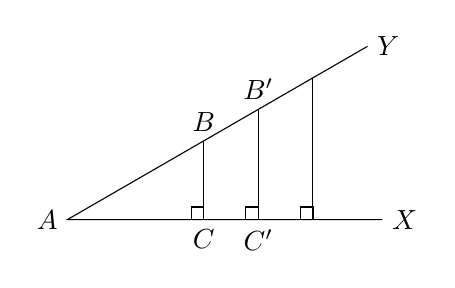
\begin{tikzpicture}[>=latex, scale=.8]
\draw(30:5.5)node[right]{$Y$}--(0,0)node[left]{$A$}--(5,0)node[right]{$X$};
\draw(30:2.5)node[above]{$B$}--+(0,-1.25)node[below]{$C$};
\draw(30:3.5)node[above]{$B'$}--+(0,-1.75)node[below]{$C'$};
\draw(30:4.5)--+(0,-2.25);
\draw(2.165,0) rectangle (2.165-.2,.2);
\draw(3.03,0) rectangle (3.03-.2,.2);
\draw(3.9,0) rectangle (3.9-.2,.2);
    \end{tikzpicture}
    \caption{}
    \end{minipage}
    \end{figure}


取任意锐角$\angle XAY$, 在边$AY$上任取一点$B$, 作$\overline{BC}\bot AX$
于$C$(图6.2). 在直角$\triangle ABC$中,设$\angle A$、$\angle B$、$\angle C$的
对边分别用$a$、$b$、$c$表示,对
锐角$A$来说,$a$叫做$\angle A$的\textbf{对
边},$b$叫做$\angle A$的相邻的直角
边(简称\textbf{邻边})我们定义:
\begin{enumerate}
    \item $\angle A$的对边与斜边的比值,叫做$\angle A$的正弦,用符
号$\sin A$来表示,即
\[\sin A=\frac{\angle A\text{的对边}}{\text{斜边}}=\frac{a}{c}\]
\item $\angle A$的邻边与斜边的比值,叫做$\angle A$的余弦。用符
号$\cos A$来表示,即
\[\cos A=\frac{\angle A\text{的邻边}}{\text{斜边}}=\frac{b}{c}\]
\item $\angle A$的对边与邻边的比值,叫做$\angle A$的正切,用符
号$\tan A$来表示,即
\[\tan A=\frac{\angle A\text{的对边}}{\angle A\text{的邻边}}=\frac{a}{b}\]
\item $\angle A$的邻边与对边的比值,叫做 $\angle A$的余切,用符
号$\cot A$来表示,即
\[\cot A=\frac{\angle A\text{的邻边}}{\angle A\text{的对边}}=\frac{b}{a}\]
\end{enumerate}

我们知道,只要$\angle A$的大
小定了,不管$B$点在边$AY$上
的位置如何(图6.3),以上
的四个比值都是不变的,只有
当$\angle A$变化时,这些比值才随着变化。这四个比都叫做锐角$A$的三角比。

有了以上定义,我们就在直角三角形的角与边之间建立
了联系,知道了角的大小,相应的四个三角比就被唯一地确
定了。反过来,如果我们知道了一个角的四个三角比中的任
何一个,我们也就能确定这个角的大小。

\begin{example}
    在直角$\triangle ABC$中,$\angle C=90^{\circ}$, $\overline{BC}=3$cm, $\overline{AC}=
    4$cm, 求$\angle A$的4个三角比(图6.4)。
\end{example}

\begin{figure}[htp]\centering
    \begin{minipage}[t]{0.48\textwidth}
    \centering
\begin{tikzpicture}[>=latex, scale=1]
\draw(0,0)node[left]{$B$}--node[below]{3}(3,0)node[right]{$C$}--node[right]{4}(3,4)node[above]{$A$}--node[left]{5}(0,0); 
\draw(3,0) rectangle (3-.2,.2);
\draw(3,4-.5) arc (-90:-36.9-90:.5);

    \end{tikzpicture}
    \caption{}
    \end{minipage}
    \begin{minipage}[t]{0.48\textwidth}
    \centering
    \begin{tikzpicture}[>=latex, scale=.8]
\draw(40:7)node[right]{$Y$}--(0,0)node[left]{$A$}--(5,0)node[right]{$X$};
\draw(4.2,0)node[below]{$C$}--node[right]{$1.8$}(4.2,3.56)node[above]{$B$};
\node at (40:3)[left]{$3$};
\node at (2.1,0)[below]{$2.1$};
\draw(4.2,0) rectangle (4,.2);
\draw(.5,0) arc (0:40:.5);
    \end{tikzpicture}
    \caption{}
    \end{minipage}
    \end{figure}

\begin{solution}
    根据勾股定理,
  \[  \overline{AB}=\sqrt{\overline{BC}^2+\overline{AC}^2}=\sqrt{3^2+4^2}=5{\rm (cm)}\]
  根据各三角比的定义有,
\[\begin{split}
    \sin A=\frac{\overline{BC}}{\overline{AB}}=\frac{3}{5},&\qquad \cos A=\frac{\overline{AC}}{\overline{AB}}=\frac{4}{5}\\
    \tan A=\frac{\overline{BC}}{\overline{AC}}=\frac{3}{4},&\qquad \cot A=\frac{\overline{AC}}{\overline{BC}}=\frac{4}{3}\\
\end{split}\]
\end{solution}


\begin{example}
      求$40^{\circ}$角的四个三角比。
\end{example}

\begin{solution}
 用量角器画$\angle XAY=40^{\circ}$(图6.5). 在边$AY$上截
取$\overline{AB}=3$cm(为计算方便,我们尽量取整数),作$\overline{BC}\bot AY$于$C$点,量得$\overline{BC}=1.8$cm, $\overline{AC}=2.1$cm, 在直角
$\triangle ABC$中,根据三角比的定义可得:
\[\sin40^{\circ}=\frac{1.8}{3}\approx 0.6,\qquad \cos40^{\circ}=\frac{2.1}{3}\approx 0.7 \]
\[\tan40^{\circ}=\frac{1.8}{2.1}\approx 0.8,\qquad \cot40^{\circ}=\frac{2.1}{1.8}\approx 1.1\]
\end{solution}

\begin{example}
    已知$\tan A=\frac{1}{2}$, 求$\angle A$.
\end{example}

\begin{figure}[htp]
    \centering
\begin{tikzpicture}
\draw(0,0)node[left]{$A$}--(4,0)node[right]{$C$}--(4,2)node[above]{$B$}--(0,0);
\draw (4,0)rectangle(4-.2,.2);
\end{tikzpicture}
    \caption{}
\end{figure}

\begin{solution}
    作一个直角$\triangle ABC$, 使直角边$\overline{AC}=2$个单位长,
$\overline{CB}=1$个单位长(图6.6),于是,
\[\tan A=\frac{1}{2}\]
用量角器量$\angle A$, 得之$\angle A\approx 26^{\circ}$。
\end{solution}

\begin{ex}
\begin{enumerate}
    \item 已知直角$\triangle ABC$, $\angle C=90^{\circ}$, $\overline{BC}=5$个单位长,$\overline{AC}=
    12$个单位长,求$\angle A$与$\angle B$的四个三角比。
    \item 用作图法求出表中各角的四个三角比的近似值,填入表
    中:
\begin{center}
    \begin{tabular}{c|cccc}
\hline
        $\alpha$ & $20^{\circ}$ & $40^{\circ}$ & $50^{\circ}$ & $80^{\circ}$\\
\hline
$\sin\alpha$\\
$\cos\alpha$\\
$\tan\alpha$\\
$\cot\alpha$\\
\hline
    \end{tabular}
\end{center}
\item 已知 $\sin\alpha=\frac{3}{4}$,
用作图法求$\angle\alpha$.
\item 已知$\cos\beta=\frac{2}{5}$,
用作图法求$\angle \beta$.
\item 已知$\tan A=\frac{3}{5}$, 
用作图法求$\angle A$.
\end{enumerate}
\end{ex}

\subsection{$0^{\circ}$到$90^{\circ}$角的三角比的变化}
半径等于1个单位长的圆叫做\textbf{单位圆}。下面我们利用单
位圆来研究锐角三角比的变化规律:

\begin{figure}[htp]
    \centering
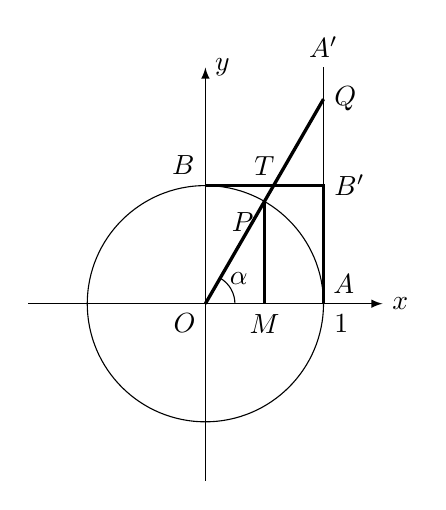
\begin{tikzpicture}[>=latex,scale=1.5]
\draw[->](-1.5,0)--(1.5,0)node[right]{$x$};
\draw[->](0,-1.5)--(0,2)node[right]{$y$};    

\draw(0,0)node[below left]{$O$} circle (1);
\draw(1,0)node[above right]{$A$}--(1,2)node[above]{$A'$};
\draw[very thick](0,0)--(60:1)node[below left]{$P$}--(60:2)node[right]{$Q$};
\draw[very thick](60:1)--(0.5,0)node[below]{$M$};
\draw[very thick](0,1)node[above left]{$B$}--(1,1)node[right]{$B'$}--(1,0)node[below right]{1};
\node at (.5,1)[above]{$T$};
\draw (.25,0) arc (0:60:.25)node[right]{$\alpha$};
\end{tikzpicture}
    \caption{}
\end{figure}


画单位圆$\odot O$(图6.7), 通过单位圆的圆心$O$作互相
垂直的两条直线,其中一条是
水平的,另一条是铅直的,以
$O$为原点,单位圆的半径为长
度单位,在两条直线上建立数
轴,其中水平轴向右为正,铅
直轴向上为正;水平轴用$x$表
示,又叫做$x$轴,铅直的轴用
$y$表示,又叫做$y$轴。以$O$为
顶点,$x$轴的正方向为一边,作$\angle AOP$等于已知角$\alpha$, $\angle AOP$
的两边分别与单位圆相交于$A$、$P$两点,过$P$点作$\overline{PM}\bot OA$于$M$点,

$\because\quad \overline{OP}=1$

$\therefore\quad \sin\alpha=\frac{\overline{MP}}{\overline{OP}}=\overline{MP}\text{的量数},\quad \cos\alpha=\frac{\overline{OM}}{\overline{OP}}=\overline{OM}\text{的量数}$

这样,对于任一锐角$\alpha$, 我们可直接用$\overline{MP}$和$\overline{OM}$的量
数来分别表示$\sin\alpha$, $\cos\alpha$的值。我们把$\overline{MP}$和$\overline{OM}$分别叫做
角$\alpha$的\textbf{正弦线}和\textbf{余弦线}。下面我们用正弦线和余弦线来研究
$\sin\alpha$与$\cos\alpha$的变化规律。

\begin{itemize}
\item 当$\alpha=0^{\circ}$时,$\overline{MP}=0$, 
$\overline{OM}=1$
\item 当$\alpha=90^{\circ}$时,$\overline{MP}=1$, 
$\overline{OM}=0$
\end{itemize}
我们就说,
\[\sin0^{\circ}=0,\qquad
\cos0^{\circ}=1,\qquad
\sin90^{\circ}=1,\qquad
\cos90^{\circ}=0.\]
我们使角$\alpha$从$0^{\circ}$逐渐增加到$90^{\circ}$, 于是从角$\alpha$的正弦线
和余弦线的变化规律可以看到,\textbf{当
$\alpha$增大时,$\sin\alpha$随着增
大,而$\cos\alpha$随着减小;反之,当$\alpha$减小时,$\sin\alpha$随着减小,
而$\cos\alpha$随着增大。}

在图6.7中,过$A$点作$AA'\bot OA$, 与角$\alpha$的一边$OP$相
交于$Q$点,于是,
\[\tan\alpha=\frac{\overline{AQ}}{\overline{OA}}=\overline{AQ}\text{的量数}\]
$\overline{AQ}$叫做角$\alpha$的\textbf{正切线}。

在图6.7中,过单位圆与$y$轴的交点$B$作$BB'\bot OB$, 角
$\alpha$的一边$OP$与$BB'$相交于$T$点,于是,
\[\cot\alpha=\frac{\overline{BT}}{\overline{OB}}=\overline{BT}\text{的量数}\]
$\overline{BT}$叫做角$\alpha$的\textbf{余切线}。

下面我们用正切线和余切线来说明角$\alpha$的正切和余切
随着角$\alpha$的变化规律。

\begin{itemize}
    \item 当$\alpha =0^{\circ}$时,$\overline{AQ}=0$, 边$OP$与$BB'$不相交,我们就说$\tan0^{\circ}=0$,
    $\cot 0^{\circ}$不存在。
    \item 当$\alpha =90^{\circ}$时,$AQ$与$OP$不相交,$\overline{BT}=0$, 
    我们就说,
    $\tan90^{\circ}$不存在,
    $\cot 90^{\circ}=0$.
\end{itemize}

我们使角$\alpha$从$0^{\circ}$增加到$90^{\circ}$, 于是从角$\alpha$的正切线和余
切线的变化规律可以看到,\textbf{当$\alpha$增大时,$\tan\alpha$也随着增大,
而$\cot\alpha$测随着减小。反之当$\alpha$减小时,$\tan\alpha$也随着减小,
而$\cot\alpha$则随着增大。}


\begin{ex}
\begin{enumerate}
    \item 在横线上填入不等号($\alpha$、$\beta$都是锐角)。
    \begin{enumerate}
    \item 当$\alpha>\beta$时,$\sin\alpha\underline{\quad}\sin\beta$,$\cos\alpha\underline{\quad}\cos\beta$,
    $\tan\alpha\underline{\quad}\tan\beta$,$\cot\alpha\underline{\quad}\cot\beta$.
    \item 当$\alpha<\beta$时,$\sin\alpha\underline{\quad}\sin\beta$,$\cos\alpha\underline{\quad}\cos\beta$,
    $\tan\alpha\underline{\quad}\tan\beta$,$\cot\alpha\underline{\quad}\cot\beta$.
    \end{enumerate}

    \item 指出下列差的符号:
\begin{multicols}{2}
\begin{enumerate}
    \item $\sin34^{\circ}-\sin33^{\circ}$
    \item $ \sin27^{\circ}-\sin26^{\circ}$
    \item $\cos83^{\circ}-\cos84^{\circ}$
    \item $\cos10^{\circ}-\cos9^{\circ}$
    \item $\tan 5^{\circ}-\tan 6^{\circ}$
    \item $\cot 14^{\circ}-\cot 13^{\circ}$
    \item $\tan 46^{\circ}-\tan 44^{\circ}$
    \item $\cot 44^{\circ}-\cot 47^{\circ}$
\end{enumerate}
\end{multicols}
\end{enumerate}
\end{ex}

\subsection{$30^{\circ}$、$45^{\circ}$、$60^{\circ}$角的三角比}
我们根据锐角三角比的定义和直角三角形中的一些边角
特殊关系,可以计算出$30^{\circ}$、$45^{\circ}$、$60^{\circ}$角的三角比的精确
值。

作$\triangle ABC$, 使$\angle C=90^{\circ}$,
$\angle A=30^{\circ}$ (图6.8), 那么
$\angle B=60^{\circ}$, 设$\overline{BC}=a$, 则$\overline{AB}=2a$, $\overline{AC}=\sqrt{\overline{AB}^2-\overline{BC}^2}=
\sqrt{(2a)^2-a^2}=\sqrt{3}a$. 
由此得:
\[\begin{split}
    \sin 30^{\circ}=\frac{a}{2a}=\frac{1}{2},&\qquad \sin 60^{\circ}=\frac{\sqrt{3}a}{2a}=\frac{\sqrt{3}}{2}\\
    \cos 30^{\circ}=\frac{\sqrt{3}a}{2a}=\frac{\sqrt{3}}{2},&\qquad \cos 60^{\circ}=\frac{a}{2a}=\frac{1}{2}\\  
\end{split}\]
\[\begin{split}
    \tan 30^{\circ}=\frac{a}{\sqrt{3}a}=\frac{1}{\sqrt{3}}=\frac{\sqrt{3}}{3},&\qquad \tan 60^{\circ}=\frac{\sqrt{3}a}{a}=\sqrt{3}\\
    \cot 30^{\circ}=\frac{\sqrt{3}a}{a}=\sqrt{3},&\qquad \cot 60^{\circ}=\frac{a}{\sqrt{3}a}=\frac{1}{\sqrt{3}}=\frac{\sqrt{3}}{3}\\  
\end{split}\]

\begin{figure}[htp]\centering
    \begin{minipage}[t]{0.48\textwidth}
    \centering
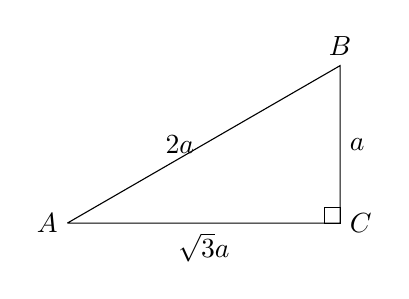
\begin{tikzpicture}[>=latex, scale=1]
     \draw(0,0)node[left]{$A$}--node[below]{$\sqrt{3}a$}(2*1.732,0)node[right]{$C$}--node[right]{$a$}(2*1.732,2)node[above]{$B$}--node[left]{$2a$}(0,0);  
     \draw(2*1.732,0)rectangle (2*1.732-.2,.2);
    \end{tikzpicture}
    \caption{}
    \end{minipage}
    \begin{minipage}[t]{0.48\textwidth}
    \centering
    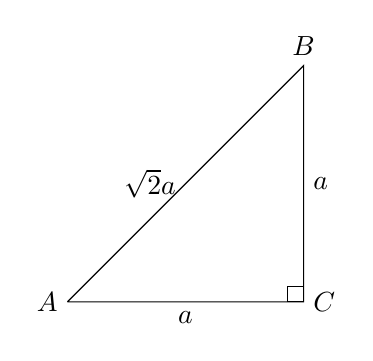
\begin{tikzpicture}[>=latex, scale=1]
 \draw(0,0)node[left]{$A$}--node[below]{$a$}(3,0)node[right]{$C$}--node[right]{$a$}(3,3)node[above]{$B$}--node[left]{$\sqrt{2}a$}(0,0);     
 \draw(3,0)rectangle (3-.2,.2);
    \end{tikzpicture}
    \caption{}
    \end{minipage}
    \end{figure}

作$\triangle ABC$, 使$\angle C=90^{\circ}$, $\angle A=45^{\circ}$ (图6.9), 那么,
$\angle B=45^{\circ}$, 设$\overline{BC}=a$, 则$\overline{AC}=a$, $\overline{AB}=\sqrt{a^2+a^2}=\sqrt{2}a$

由此得:
\[\sin 45^{\circ}=\frac{a}{\sqrt{2}a}=\frac{1}{\sqrt{2}}=\frac{\sqrt{2}}{2},\qquad \cos 45^{\circ}=\frac{a}{\sqrt{2}a}=\frac{1}{\sqrt{2}}=\frac{\sqrt{2}}{2}\]
\[\tan 45^{\circ}=\frac{a}{a}=1,\qquad \cot 45^{\circ}=\frac{a}{a}=1\]
为了便于记忆,我们把$30^{\circ},45^{\circ},60^{\circ}$的三角比列成表。
\begin{center}
    \begin{tabular}{c|ccc}
        \hline
$\alpha$&$30^{\circ}$&$45^{\circ}$&$60^{\circ}$\\
\hline
$\sin\alpha$  &  $\frac{1}{2}$ & $\frac{\sqrt{2}}{2}$& $\frac{\sqrt{3}}{2}$\\
$\cos\alpha$  &  $\frac{\sqrt{3}}{2}$ & $\frac{\sqrt{2}}{2}$& $\frac{1}{2}$\\
$\tan\alpha$  &  $\frac{\sqrt{3}}{3}$ &1&$\sqrt{3}$\\
$\cot\alpha$  &  $\sqrt{3}$ &1&$\frac{\sqrt{3}}{3}$\\
\hline
    \end{tabular}
\end{center}

\begin{example}
    计算 $4\cot 30^{\circ}-2\sin60^{\circ}+2\cos60^{\circ}$
\end{example}

\begin{solution}
\[4\cot 30^{\circ}-2\sin60^{\circ}+2\cos60^{\circ} =4\x \sqrt{3}-2\x \frac{\sqrt{3}}{2}+2\x \frac{1}{2}=3\sqrt{3}+1
\]
\end{solution}


\begin{example}
    计算
$\cos^2 30^{\circ}+\sin^2 45^{\circ}-\tan^2 45^{\circ}$
其中:$\sin^\alpha$、$\cos^2\alpha$
$\tan^2\alpha$、$\cot^2\alpha$分别表示$(\sin\alpha)^2$、$(\cos \alpha)^2$、$(\tan\alpha)^2$、$(\cot \alpha)^2$
\end{example}


\begin{solution}
\[\cos^2 30^{\circ}+\sin^2 45^{\circ}-\tan^2 45^{\circ}=\left(\frac{\sqrt{3}}{2}\right)^2+\left(\frac{\sqrt{2}}{2}\right)^2-1^2=\frac{3}{4}+\frac{2}{4}-1=\frac{1}{4}\]
\end{solution}

\begin{ex}
    求下列各式之值:
\begin{enumerate}
\item $\sin^2 60^{\circ}+\cos^2 30^{\circ}$
\item $\sin^2 60^{\circ}+\cos^2 60^{\circ}$
\item $\sin^2 45^{\circ}+\cos^2 45^{\circ}$
\item $2\sin30^{\circ}+2\cos60^{\circ}+4\tan 45^{\circ}$
\item $5\tan 30^{\circ}+\cot 45^{\circ}-2\tan 45^{\circ}+2\cos 60^{\circ}$  
\item $\frac{2\sin30^{\circ}}{2\cos30^{\circ}-1}$
\item $\frac{\sin60^{\circ}-\sin30^{\circ}}{\sin60^{\circ}+\sin30^{\circ}}$
\end{enumerate}
\end{ex}

\subsection{三角比值表}
在前面的内容中,我们讲的只是特殊角的三角比,为了应用方
便,人们早已制定了任意锐角的三角比值表,下面就来介绍
四位三角比值表的用法。

\subsubsection{正弦表,余弦表}
在正弦、余弦表里左右各有一列排度数,左列上端和右
列下端都有$A$字,在左列$A$的下面,由上到下排着度数,
在右列$A$的上面,由下到上排着度数,在顶行$A$的右边,
由左至右依次排着$0',6',\ldots,60'$, 在表的顶上写着正弦表,
说明查正弦时用左列$A$下面的度数和顶行的分数,表的底下
写着余弦表,说明查余弦时,用右列$A$上的度数和底行的分
数。例如要查$26^{\circ}18'$的正弦,在表中左列$A$的下面先找到
$26^{\circ}$, 顺着$26^{\circ}$所在的这一行往右,在顶行$18'$所在的这一列
里找到了一个数0.4431, 就是$26^{\circ}18'$的正弦,即$\sin26^{\circ}18'=
0.4431$. 换句话说左列$A$下面的$26^{\circ}$所在的行和顶行$18'$所
在的列的交点处的0.4431, 就是$\sin26^{\circ}18'$. 要查$\cos27^{\circ}24'$, 
在表中右列$A$的上面找到$27^{\circ}$, 底行里找到$24'$, $27^{\circ}$所在的
行和$24'$所在的列的交点处的0.8878, 就是$\cos27^{\circ}24'$, 即
$\cos27^{\circ}24'=0.8878$.

\subsubsection{正切表、余切表}
正切的查法和正弦相同,余切的查法和余弦相同,例如
我们在正切表、余切表中可以查到:
\[\tan 54^{\circ}30'=1.4019,\qquad \cot 4^{\circ}6'=13.95\]

\begin{ex}
    查表求下列各三角比:
\begin{enumerate}
    \item $\sin14^{\circ},\quad \sin20^{\circ}24',\quad \sin65^{\circ}30',\quad \sin82^{\circ}12'$
    \item $\cos7^{\circ},\quad  \cos32^{\circ}6',\quad  \cos60^{\circ}54',\quad \cos83^{\circ}18'$
    \item $\tan 18^{\circ},\quad  \tan 78^{\circ}36',\quad  \tan 80^{\circ}24',\quad  \tan 83^{\circ}$
    \item $\cot 42^{\circ}42',\quad   \cot20^{\circ}48', \quad  \cot9^{\circ}36', \quad  \cot 5^{\circ}30'$
\end{enumerate}
\end{ex}

在三角比值表中,最右边的三列是修正值,它是用来求
在左边表里找不到的角的三角比,这三列的上端和下端都标
有$1'$、$2'$、$3'$, 三列中的数是小数的简写,每一个数都代表
一个小数,它的末位数相当于表中间同一行小数的末位数,
$1'$、$2'$、$3'$各列中的各数,分别是它所在的行的角度分别相
差$1'$、$2'$、$3'$时的三角比的修正值,下面举列说明查法:

例如,要求$\sin20^{\circ}19'$, 先从表中查得$\sin20^{\circ}18'$的值是
0.3469, 因为$20^{\circ}19'$比$20^{\circ}18'$大$1'$, 查修正值是0.0003. 因
为角度大,它的正弦值也大,所以$\sin20^{\circ}19'$就比$\sin20^{\circ}18'$
大0.0003, 因此,$\sin20^{\circ}19'=0.3469+0.0003=0.3472$. 要
求$\sin20^{\circ}46'$, 先从表中查得$\sin20^{\circ}48'$的值是0.3551, $20^{\circ}46'$
比$20^{\circ}48'$小$2'$, 查得$2'$的修正值是0.0005, 角度小,正弦值
也小,所以$\sin20^{\circ}46'=0.3551-0.0005=0.3546$. 要求
$\cos28^{\circ}26'$, 先从表中查得$\cos28^{\circ}24'=0.8796$, $28^{\circ}26'$比
$28^{\circ}24'$大$2'$, 查表得修正值是0.0003, 角大余弦值反而小,
所以$\cos28^{\circ}26'=0.8796-0.0003=0.8793$. 

正切的查法和正弦相同,余切的查法和余弦相同。

例如,我们可以求得
\[\tan 69^{\circ}25'=2.662,\qquad \cot 70^{\circ}45'=0.3492\]

\begin{ex}
    查表求下列各三角函数:
\begin{multicols}{2}
    \begin{enumerate}
        \item $\sin18^{\circ}19',\quad  \sin63^{\circ}40'$
        \item $\cos65^{\circ}2',\quad  \cos10^{\circ}34'$
        \item $\tan 9^{\circ}19',\quad  \tan64^{\circ}10'$
        \item $\cot25^{\circ}28',\quad  \cot10^{\circ}25'$
    \end{enumerate}
\end{multicols}
\end{ex}

从三角比值表里不但可以查得任何锐角的三角比,反过
来,也可以根据已知的三角比值查到未知的锐角。

\begin{example}
    已知$\sin x=0.9966$, 求锐角
    $x$.
\end{example}

\begin{solution}
    在正弦表里找到0.9966, 因为它是正弦的值,要用到左
    列的度和顶行的分,在0.9966这一行的左端是$85^{\circ}$, 在0.5966
    的上端是$18'$. 所以
   $ \sin85^{\circ}18'=0.9966$, 因此$x=85^{\circ}18'$.
\end{solution}

\begin{example}
已知$\cos y=0.9966$, 求锐角$y$.
\end{example}

\begin{solution}   
    在表中找到0.9966, 因为它是余弦的值,余弦要用到右
    列的度数和底行的分,在0.9966这一行的右端是$4^{\circ}$, 在
    0.9966这一列的下端是$42'$.

    所以$\cos4^{\circ}42'=0.9966$, 因此$y=4^{\circ}42'$.
\end{solution}

\begin{example}
   $\tan x=14.30$, $\cot y=1.4715$, 求$x$、$y$. 
\end{example}

\begin{solution}
    倒查正切表(查法和例6.6相同)可得:$x=86^{\circ}$.

倒查余切表(查法和例6.7相同)可得:$y=34^{\circ}12'$.
\end{solution}

由三角比值求角度,有时要用到修正值,用修正值时,
必须注意到,对于正弦、正切的值越大,角度也越大;对于
余弦、余切的值越大,角度反而越小,下面举例说明用修正
值查法。

\begin{example}
      $\sin x=0.2493$, 求$x$.
\end{example}

\begin{solution}
在正弦表里,和0.2493最接近的正弦值是0.2487, 它是
$14^{\circ}24'$的正弦,$0.2493-0.2487=0.0006$, 在$14^{\circ}$这一行里
正弦值相差0.0006时,角度的修正值是$2'$, $\sin x$比$\sin14^{\circ}24'$
大0.0006, $x$就比$14^{\circ}24'$大$2'$, 因此
\[x=14^{\circ}24'+2'=14^{\circ}26'\]
\end{solution}

\begin{example}
    $\cos y=0.9841$, 求$y$.
\end{example}

\begin{solution}
    在余弦表中和0.9841最接近的余弦值是0.9842, 它是
$10^{\circ}12'$的余弦,$0.9842-0.9841=0.0001$, 在$10^{\circ}$这一行里
余弦值相差0.0001时,角度的修正值是$1'$或$2'$, $\cos y$比
$\cos10^{\circ}12'$小0.0001, $y$比$12^{\circ}12'$大$1'$或$2'$, 因此
\[y=10^{\circ}12'+1'=10^{\circ}13'\]
或\[y=10^{\circ}12'+2'=10^{\circ}14'\]
这里$y$有两个答案,
一个是不足近似值,一个过剩近似值。
\end{solution}

\begin{example}
    $\tan x=1.3773$, $\cot=0.1950$, 求$x$、$y$.
\end{example}

\begin{solution}
倒查正切表,得$x=54^{\circ}1'$(查法和例6.9相同)。

倒查余切表,得$y=78^{\circ}51'$(查法和例6.10相同)。
\end{solution}

\begin{ex}
    由三角比值表求锐角$x$:
\begin{enumerate}
    \item $\sin x=0.9816,\quad
    \sin x=0.6639,\quad
    \tan x=9.595,\quad
    \tan x=0.1890$
    \item $\cos x=0.8607,\quad
    \cos x=0.9893,\quad
    \cot x=2.106,\quad
    \cot x=67.40$
    \item $\sin x=0.2476,\quad
    \sin x=0.9709,\quad
    \cos x=0.3372$
    
    $
    \cos x=0.4174,\quad
    \tan x=0.365,\quad
    \cot x=0.1614$
\end{enumerate}
\end{ex}

\subsection{互为余角的三角比间的关系}
\begin{figure}[htp]
    \centering
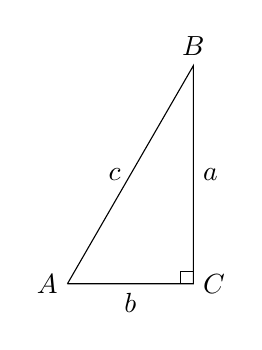
\begin{tikzpicture}[>=latex, scale=.8]
     \draw(0,0)node[left]{$A$}--node[below]{$b$}(2,0)node[right]{$C$}--node[right]{$a$}(2,2*1.732)node[above]{$B$}--node[left]{$c$}(0,0);  
     \draw(2,0)rectangle (2-.2,.2);
    \end{tikzpicture}
    \caption{}
\end{figure}

在直角$\triangle ABC$中,如果$\angle C=90^{\circ}$(图6.10), 则
\[\angle A+\angle B=90^{\circ},\qquad \angle B=90^{\circ}-\angle A\]
由于$\angle A$的对边是$\angle B$的邻边,
$\angle B$的对边是$\angle A$的邻边,那么,根
据三角比的定义,我们便得出$\angle A$和
$\angle B$这两个互为余角的三角比之间有
下面的关系:
\[\begin{split}
    \sin A=\frac{a}{c}=\cos B=\cos(90^{\circ}-A),&\qquad \cos A=\frac{b}{c}=\sin B=\sin(90^{\circ}-A)\\
    \tan A=\frac{a}{b}=\cot B=\cot(90^{\circ}-A),&\qquad \cot A=\frac{b}{a}=\tan B=\tan(90^{\circ}-A)\\
\end{split}\]

这就是说,\textbf{互为余角的两个角中,任一角的正弦等于另
一角的余弦;任一角的正切等于另一角的余切。}

有了这个关系,我们就可把任意大于$45^{\circ}$的锐角的三角
比化为小于$45^{\circ}$的锐角的三角比。

\begin{example}
    把下面各角的三角比化为小于$45^{\circ}$的锐角的三角
    比。
\begin{multicols}{2}
\begin{enumerate}
\item $\sin75^{\circ}$
\item $\cos62^{\circ}22'$
\item $\tan 80^{\circ}$
\item $\cot56^{\circ}18'$
\end{enumerate}
\end{multicols}
\end{example}

\begin{solution}
\begin{enumerate}
    \item $\sin75^{\circ}=\cos(90^{\circ}-75^{\circ})=\cos 15^{\circ}$
    \item $\cos62^{\circ}22'=\sin(90^{\circ}-62^{\circ}22')=\sin27^{\circ}38'$
    \item $\tan 80^{\circ}=\cot(90^{\circ}-80^{\circ})=\cot10^{\circ}$
    \item $\cot 56^{\circ}18'=\tan(90^{\circ}-56^{\circ}18')=\tan 33^{\circ}42'$
\end{enumerate}
\end{solution}


\begin{example}
    下列等式是否成立:
\begin{enumerate}
\item $\sin(60^{\circ}+\alpha )=\cos(30^{\circ}-\alpha ) \qquad (0\le \alpha \le 30^{\circ})$
\item $\sin(45^{\circ}+\alpha )=\cos(45^{\circ}-\alpha ) \qquad (0\le \alpha \le 45^{\circ})$
\item $\tan(50^{\circ}+\alpha )=\cot (40^{\circ}-\alpha ) \qquad (0\le \alpha <40^{\circ})$
\end{enumerate}
\end{example}


\begin{solution}
由于
\[\begin{split}
    (60^{\circ}+\alpha )+(30^{\circ}-\alpha )&=90^{\circ}\\
(45^{\circ}+\alpha )+(45^{\circ}-\alpha )&=90^{\circ}\\
(50^{\circ}+\alpha )+(40^{\circ}-\alpha )&=90^{\circ}
\end{split}\]

而$\alpha $角的取值范围使得各式中的三角比都有意义,所以
根据互为余角的三角比之间的关系可知,各等式都成立。
\end{solution}

\begin{ex}
    \begin{enumerate}
        \item 为什么三角比值表中,锐角$\alpha$的正弦和$90^{\circ}-\alpha$角的余弦共
        用一个表。
\item 把下列各角的三角比化为小于$45^{\circ}$的锐角的三角比。
\begin{multicols}{2}
\begin{enumerate}
    \item $\sin73^{\circ},\qquad \sin77^{\circ}18'$
    \item $\cos57^{\circ},\qquad \cos52^{\circ}38'$
    \item $\tan78^{\circ},\qquad \tan79^{\circ}5'$
    \item $\cot48^{\circ},\qquad \cot78^{\circ}31'$
\end{enumerate}
\end{multicols}
\item 下列各式中的$x$应为多少度?
\begin{multicols}{2}
\begin{enumerate}
    \item $\sin75^{\circ}=\cos x$
    \item $\cos18^{\circ}=\sin x$
    \item $\tan5^{\circ}=\cot x$
    \item $\cot83^{\circ}=\tan x$
\end{enumerate}
\end{multicols}
\item 下列等式是否成立($x$、$\alpha$的取值都使各三角比有意义)。
\begin{multicols}{2}
\begin{enumerate}
    \item $\sin(75^{\circ}+\alpha )=\cos(15^{\circ}-\alpha )$
    \item $\sin(15^{\circ}-\alpha )=\sin(30^{\circ}+\alpha )$
    \item $ \tan (30^{\circ}+x)=\cot (60^{\circ}-x)$
    \item $ \cot (89^{\circ}+\alpha )=\tan (1^{\circ}-\alpha )$
\end{enumerate}
\end{multicols}
    \end{enumerate}
\end{ex}

\subsection{同一锐角的各三角比间的关系}
\begin{blk}{定理}
    同一锐角$\alpha$ 的四个三角比之间有下列关系:
\begin{enumerate}
    \item $\sin^2\alpha  +\cos^2\alpha =1$
    \item $\tan\alpha=\frac{\sin\alpha}{\cos\alpha },\qquad \cot\alpha=\frac{\cos\alpha }{\sin\alpha }$
    \item $\tan\alpha\cdot \cot\alpha =1$
\end{enumerate}
\end{blk}

\begin{proof}
    作直角$\triangle ABC$, 使$\angle C=90^{\circ}$, $\angle A=\alpha$ (图6.11).
    \begin{figure}[htp]
        \centering
    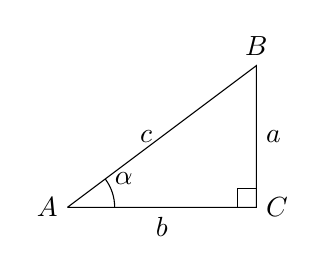
\begin{tikzpicture}[>=latex, scale=1.2]
         \draw(0,0)node[left]{$A$}--node[below]{$b$}(2,0)node[right]{$C$}--node[right]{$a$}(2,1.5)node[above]{$B$}--node[left]{$c$}(0,0);  
         \draw(2,0)rectangle (2-.2,.2);
         \draw (.5,0) arc (0:36.87:.5)node[right]{$\alpha$};
        \end{tikzpicture}
        \caption{}
    \end{figure}
    
\begin{enumerate}
    \item $\because\quad  a^2+b^2=c^2$
    
    $\therefore\quad \left(\frac{a}{c}\right)^2+\left(\frac{b}{c}\right)^2=1$

    又$\because\quad \frac{a}{c}=\sin\alpha,\quad \frac{b}{c}=\cos\alpha$,

    $\therefore\quad \sin^2\alpha  +\cos^2\alpha =1$,即:
\textbf{一锐角的正弦和余弦的平方和等于1.}
该式也就是勾股定理的三角比的表示式。

\item $\because\quad \tan\alpha=\frac{a}{b},\quad \frac{\sin\alpha}{\cos\alpha}=\frac{\frac{a}{c}}{\frac{b}{c}}=\frac{a}{b}$,

$\therefore\quad \tan\alpha=\frac{\sin\alpha}{\cos\alpha}$

又$\because\quad \cot\alpha=\frac{b}{a},\quad \frac{\cos\alpha}{\sin\alpha}=\frac{\frac{b}{c}}{\frac{a}{c}}=\frac{b}{a}$,

$\therefore\quad \cot\alpha=\frac{\cos\alpha}{\sin\alpha}$

\item $\because\quad \tan\alpha=\frac{a}{b},\quad \cot\alpha=\frac{b}{a}$

$\therefore\quad \tan\alpha\cdot \cot\alpha=\frac{a}{b}\cdot \frac{b}{a}=1$
\end{enumerate}
\end{proof}

上面的定理,表示了同一锐角的三角比之间的关系,我
们可利用定理中的三个公式,由已知锐角的一个三角比,去
计算这个角的其它的三个三角比;也可以利用它们来化简含
有三角比的式子。


\begin{example}
    已知:$\sin\alpha=\frac{3}{5}$, 
    求$\alpha$角($\alpha$为锐角)的其它
    的三个三角比。
\end{example}


\begin{solution}
 从公式$\sin^2\alpha +\cos^2\alpha =1$ 可得
   \[ \cos\alpha =\pm\sqrt{1-\sin^2\alpha}\] 
   由于锐角的三角比都是正
    数,所以根号前应取正号,把$\sin\alpha =\frac{3}{5}$
    代入上式,得
\[\cos\alpha=\sqrt{1-\left(\frac{3}{5}\right)^2}=\sqrt{\frac{25-9}{5^2}}=\frac{4}{5}\]
根据$\tan\alpha=\frac{\sin\alpha}{\cos\alpha}$,可得
\[\tan\alpha=\frac{\frac{3}{5}}{\frac{4}{5}}=\frac{3}{4}\]
再根据$\tan\alpha\cdot \cot\alpha=1$,可得
\[\cot\alpha=\frac{4}{3}\]
\end{solution}

\begin{example}
    化简
    $\sin^2 54^{\circ}+\sin^2 36^{\circ}-\tan 45^{\circ}$
\end{example}

\begin{solution}
\[\begin{split}
    \sin^2 54^{\circ}+\sin^2 36^{\circ}-\tan 45^{\circ}&=
    \cos^2(90^{\circ}-54^{\circ})+\sin^2 36^{\circ}-\tan 45^{\circ}\\
    &=\cos^2 36^{\circ}+\sin^2 36^{\circ}-1\\
    &=1-1=0
\end{split}\]
\end{solution}


\begin{example}
    化简$\frac{\sqrt{1-\sin^2\alpha}}{\sin\alpha}\cdot \tan\alpha$
\end{example}

\begin{solution}
    \[\frac{\sqrt{1-\sin^2\alpha}}{\sin\alpha}\cdot \tan\alpha=\frac{\cos\alpha}{\sin\alpha}\cdot \tan\alpha=\cot\alpha\cdot \tan\alpha=1\]
\end{solution}

\begin{example}
    化简$(\sin\alpha+\cos\alpha)^2+(\sin\alpha-\cos\alpha)^2$
\end{example}

\begin{solution}
\[\begin{split}
&    (\sin\alpha+\cos\alpha)^2+(\sin\alpha-\cos\alpha)^2\\  
&\quad =\sin^2\alpha+2\sin\alpha\cdot \cos\alpha+\cos^2\alpha
+\sin^2\alpha-2\sin\alpha\cdot\cos\alpha+\cos^2\alpha\\
&\quad =1+1=2
\end{split}\]    
\end{solution}

\begin{ex}
\begin{enumerate}
    \item 证明$\sin^2\alpha+\cos^2\alpha=1$, $\tan\alpha=\frac{\sin\alpha}{\cos\alpha}$
    \item 已知$\sin\alpha=\frac{5}{13}$,求$\cos\alpha, \tan\alpha, \cot\alpha$
    \item 已知$\cos\alpha=\frac{4}{5}$,求$\sin\alpha, \tan\alpha, \cot\alpha$
    \item 已知$\tan\alpha=\frac{3}{4}$,求$\sin\alpha,\cos\alpha$。
    
提示:$\tan^2\alpha =\frac{\sin^2\alpha}{1-\sin^2\alpha}=\frac{9}{16}$,令$\sin \alpha =x$,解方程。

\item 化简

\begin{enumerate}\begin{multicols}{2}
    \item $\frac{1-\sin^2\alpha}{\cos^2\alpha}$
    \item $\tan\alpha\cdot \cos\alpha$
    \item $\frac{\cos\alpha}{\sqrt{1-\cos^2\alpha}}$
    \item $\frac{\sin^2\alpha}{1+\cos\alpha}$
    \item $\frac{\cos^2\alpha}{1-\sin\alpha}$\end{multicols}
    \item $(\tan\alpha+\cot\alpha)^2-(\tan\alpha-\cot\alpha)^2$
\end{enumerate}

\end{enumerate}
\end{ex}

\subsection*{习题6.1}
\begin{enumerate}
    \item 在直角$\triangle ABC$中,$\angle C=90^{\circ}$, $a=3$, $b=2$, 求$\angle A$的四
    个三角比。
    \item 在直角$\triangle ABC$中,$\angle C=90^{\circ}$,$\overline{AB}=10$, $\overline{BC}=8$, 求:
   $ \sin A$、$\cos A$.
    \item 在直角$\triangle ABC$中,$\angle C=90^{\circ}$, $\overline{CD}$为$\overline{AB}$边上的高,问
    图中哪些线段的比可以表
    示$\angle A$的正弦?哪些线段
    的比可以表示$\angle B$的正弦?
\begin{figure}[htp]
    \centering
    \begin{tikzpicture}
\draw(0,0)node[below]{$A$}--(5,0)node[below]{$B$}--(3.2,2.4)node[above]{$C$}--(0,0);
\draw(3.2,2.4)--(3.2,0)node[below]{$D$};
\draw(3.2,0) rectangle (3.2+.2,.2);        
\draw (0.4,0) arc (0:32:.4);
\draw (3.2,2) arc (-90:-90+32:.4);
    \end{tikzpicture}
    \caption*{第3题}
\end{figure}

    \item 判断下列等式是否正确:
\begin{enumerate}
\item $\sin35^{\circ} 30'=\cos54^{\circ} 30'$
\item $\sin(30^{\circ} -\alpha )=\cos(60^{\circ} +\alpha )$
\item $\cos(2\alpha +14^{\circ} )=\sin(76^{\circ} -2\alpha )$
\end{enumerate}

\item 化简下列各式:
\begin{enumerate}
\item $\sin^4\alpha  +2\sin^2\alpha \cos^2\alpha +\cos^4\alpha $
\item $\sin^4\alpha -\cos^4\alpha +\cos^2\alpha $
\item $\sin(45^{\circ} +\alpha )-\cos(45^{\circ} -\alpha )$    
\item $\frac{1-\sin^2\alpha }{1-\cos^2\alpha }$
\item $\frac{\tan \alpha +\tan \beta}{\cot\alpha +\cot \beta}$
\item $\sin(90^{\circ} -\alpha )\cdot \cot(90^{\circ} -\alpha )$
\end{enumerate}

\item 已知 $\tan \alpha =2$, 求 $\tan(90^{\circ} -\alpha )$.
\item 已知
$\sin A=\frac{1}{3}$
求 $\cos A$, $\tan A$.
\item 已知互为余角的两角的正切的和等于3, 求两角正切的
平方和。
\item 求下列各题中的未知锐角$x$:
\begin{multicols}{2}
\begin{enumerate}
    \item $\sin x=\frac{1}{2}$
    \item $\cos x=\frac{\sqrt{2}}{2}$
    \item $\tan x=\sqrt{3}$
    \item $\sin x=\frac{\sqrt{3}}{2}$
    \item $\cos x=\frac{1}{2}$
    \item $\tan x=\frac{1}{\sqrt{3}}$
\end{enumerate}
\end{multicols}

\item 已知 $\cos^2 x=\frac{1}{4}$,求$x$.
\item 已知 $\cos^2x-\sin^2x=\frac{1}{2}$, 
求$x$.
\item 回答下列问题:
\begin{enumerate}
\item 当$0^{\circ}\le \alpha\le 90^{\circ}$时,$\sin\alpha$的最大值是多少?最小值
是多少?
\item 当$0^{\circ}\le \alpha\le 90^{\circ}$时,$\cos\alpha$的最大值是多少?最小值
是多少?
\end{enumerate}


\item 当$0^{\circ}\le \alpha\le 45^{\circ}$, $\alpha=45^{\circ}$, $45^{\circ}<\alpha\le 90^{\circ}$时,分别比较
$\sin\alpha$与$\cos\alpha$的大小。
\end{enumerate}

\section{解直角三角形}
\subsection{直角三角形中的边角关系}

我们把学过的直角三角形中
的边角基本关系总结如下:
\begin{figure}[htp]
    \centering
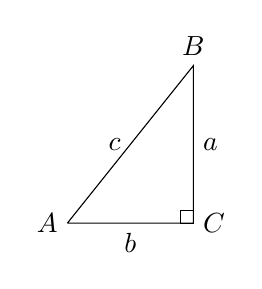
\begin{tikzpicture}[>=latex, scale=.8]
     \draw(0,0)node[left]{$A$}--node[below]{$b$}(2,0)node[right]{$C$}--node[right]{$a$}(2,2.5)node[above]{$B$}--node[left]{$c$}(0,0);  
     \draw(2,0)rectangle (2-.2,.2);
    \end{tikzpicture}
    \caption{}
\end{figure}

已知$\triangle ABC$, $\angle C=90^{\circ}$ (图6.12).
\begin{enumerate}
    \item 勾股定理:$a^2+b^2=c^2$
    \item 两锐角互余:$\angle A+\angle B=90^{\circ}$
    \item 四个三角比:
\[\sin A=\frac{\angle A\text{的对边}}{\angle A\text{斜边}},\qquad \cos A=\frac{\angle A\text{的邻边}}{\angle A\text{斜边}}\]
\[\tan A=\frac{\angle A\text{的对边}}{\angle A\text{的邻边}},\qquad \cot A=\frac{\angle A\text{的邻边}}{\angle A\text{的对边}}\]
\end{enumerate}
    为了应用方便,我们把3中的四个公式写成下面的形
    式:
\[\angle A\text{的对边}=\text{斜边}\x \sin A,\qquad \angle A\text{的邻边}=\text{斜边}\x \cos A\]
\[\angle A\text{的对边}=\text{邻边}\x \tan A,\qquad \angle A\text{的邻边}=\text{对边}\x \cot A\]

改用语言叙述,就是:
\begin{blk}{}
 在直角三角形中:
\begin{enumerate}
\item 一条直角边等于斜边乘上这条直角边所对锐角的
正弦。
\item 一条直角边等于斜边乘上这条直角边相邻锐角的
余弦。
\item 一条直角边等于另一条直角边乘上这条直角边所
对锐角的正切。
\item 一条直角边等于另一条直角边乘上这条直角边相
邻锐角的余切。
\end{enumerate}
\end{blk}

\begin{ex}
    \begin{enumerate}
        \item 在直角$\triangle ABC$中,$\angle C=90^{\circ}$, 求证:
\[\overline{AB}=\frac{\overline{BC}}{\sin A},\qquad \overline{AB}=\frac{\overline{AC}}{\cos A}\]
       并把这两个式子用语言叙述出来。
        \item 在直角$\triangle ABC$中,$\angle C=90^{\circ}$,求证:
\begin{enumerate}
    \item $\sin A=\cos B,\qquad      \sin B=\cos A$
    \item $\tan A=\cot B,\qquad \cot A=\tan B$
\end{enumerate}
    \end{enumerate}

\end{ex}

\subsection{解直角三角形}
根据三角形的某些已知元素求出它的未知元素,这种过
程叫做\textbf{解三角形}。在直角三角形中,直角总是已知的。除直
角外,只要再知道两个元素,其中至少有一边,就可以求出
直角三角形的其它各元素。因此,解直角三角形,只有下面
四种情况:
\begin{enumerate}
    \item 已知斜边与一锐角,
    \item 已知一条直角边与一锐角;
    \item 已知斜边与一条直角边;
    \item 已知两条直角边。
\end{enumerate}

上述四种情况,都可用前面中所列出的关系式,并利用
三角比值表来求解。

\begin{example}
    已知$c=18$, $\angle A=62^{\circ}20'$ (图6.13),
求:$\angle B, a, b$
\end{example}

\begin{solution}
\[\begin{split}
    \angle B&=90^{\circ}-\angle A=90^{\circ}-62^{\circ}20'
=27^{\circ}40'\\
a&=c\sin A=18\x \sin62^{\circ}20'=18\x0.8857
\approx 15.9\\
b&=c\cos A=18\x\cos62^{\circ}20'=18\x0.4643\approx 8.3600
\end{split}\]
\end{solution}

\begin{figure}[htp]\centering
    \begin{minipage}[t]{0.48\textwidth}
    \centering
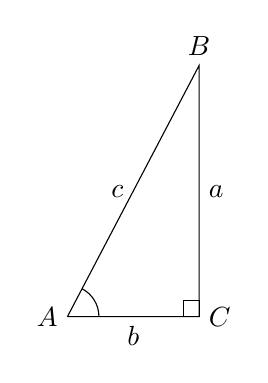
\begin{tikzpicture}[>=latex, scale=2]
    \draw(0,0)node[left]{$A$}--node[below]{$b$}(.8358,0)node[right]{$C$}--node[right]{$a$}(62.33:1.8)node[above]{$B$}--node[left]{$c$}(0,0);  
    \draw(.8358,0)rectangle (.8358-.1,.1);
    \draw(.2,0) arc (0:62.33:.2);
    \end{tikzpicture}
    \caption{}
    \end{minipage}
    \begin{minipage}[t]{0.48\textwidth}
    \centering
    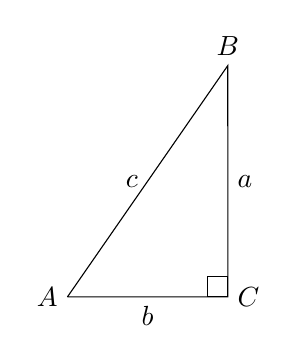
\begin{tikzpicture}[>=latex, scale=1.3]
\draw(0,0)node[left]{$A$}--node[below]{$b$}(1.567,0)node[right]{$C$}--node[right]{$a$}(55.27:2.75)node[above]{$B$}--node[left]{$c$}(0,0);  
    \draw(1.567,0)rectangle (1.567-.2,.2);
    \end{tikzpicture}
    \caption{}
    \end{minipage}
    \end{figure}

\begin{example}
    已知$c=27.5$, $a=22.6$, 求$b$、$\angle A$、$\angle B$ (图6.14).
\end{example}

\begin{solution}
\[b=\sqrt{c^2-a^2}=\sqrt{27.5^2-22.6^2}\approx 15.7\]
由于
$\sin A=\frac{a}{c}=\frac{22.6}{27.5}\approx 0.8218$,
因此:
\[\begin{split}
    \angle A&\approx 55^{\circ}16'\\
\angle B&=90^{\circ}-\angle A=90^{\circ}-55^{\circ}16'=34^{\circ}44'
\end{split}\]
\end{solution}


\begin{example}
    已知$a=3.8$, $\angle A=42^{\circ}$, 求$\angle B$, $C$, $b$ (图6.15).
\end{example}

\begin{solution}
\[\begin{split}
    B&=90^{\circ} -\angle A=48^{\circ} \\
b&=a \cot A=3.8\x\cot 42^{\circ}\approx 4.22\\
c&=\frac{a}{\sin A}=\frac{3.8}{\sin 42^{\circ}}\approx 5.68 
\end{split}\]
    
\end{solution}

\begin{figure}[htp]\centering
    \begin{minipage}[t]{0.48\textwidth}
    \centering
\begin{tikzpicture}[>=latex, scale=.7]
    \draw(0,0)node[left]{$A$}--node[below]{$b$}(4.22,0)node[right]{$C$}--node[right]{$a$}(42:5.68)node[above]{$B$}--node[left]{$c$}(0,0);  
    \draw(4.22,0)rectangle (4.22-.2,.2);
    \draw(.6,0) arc (0:42:.6);
    \end{tikzpicture}
    \caption{}
    \end{minipage}
    \begin{minipage}[t]{0.48\textwidth}
    \centering
    \begin{tikzpicture}[>=latex, scale=.8]
\draw(0,0)node[left]{$B$}--node[below]{$c$}(5,0)node[right]{$A$}--node[right]{$b$}(90-36.87:3)node[above]{$C$}--node[left]{$a$}(0,0);  
  
    \end{tikzpicture}
    \caption{}
    \end{minipage}
    \end{figure}


\begin{example}
    已知$a=3$、$b=4$, 求$c$、$\angle A$、$\angle B$ (图6.16)
\end{example}

\begin{solution}
\[c=\sqrt{a^2+b^2}=\sqrt{3^2+4^2}=5\]
由于$\tan A=\frac{3}{4}=0.75$,
因此:$$\angle A\approx 36^{\circ} 52',\qquad 
\angle B\approx 90^{\circ} -36^{\circ} 52'=53^{\circ} 8'$$ 
\end{solution}

\begin{ex}
\begin{enumerate}
    \item 解下列直角三角形:
    \begin{enumerate}
    \item 已知$c=58.5,\quad \angle A=45^{\circ} 13'$
    \item 已知$c=14,\quad \angle B=62^{\circ}$
    \item 已知$c=28,\quad \angle A=34^{\circ} $
    \item 已知$c=195,\quad \angle B=78^{\circ} 47'$
    \item 已知$a=87,\quad \angle A=55^{\circ} $
    \item 已知$b=99,\quad \angle B=83^{\circ} $
    \item 已知$c=32,\quad a=18$
    \item 已知$a=14,\quad \angle B=78^{\circ}$
    \item 已知$c=79,\quad b=56$
    \item 已知$a=12.8,\quad b=15.6$
    \item 已知$c=73,\quad \angle B=66.2^{\circ}$ 
    \item 已知$c=350,\quad \angle A=3.8^{\circ} $
\end{enumerate}

\item 已知直角$\triangle ABC$, $\angle C=90^{\circ}$, $\angle A=\alpha$和$\angle A$对的直角边是
$a$

求证:直角$\triangle ABC$的面积$S=\frac{a^2}{2}\tan\alpha$

\item  已知直角三角形的一个锐角为$\alpha$, 面积等于$S$, 
求它的外接圆的面积。
\end{enumerate}
\end{ex}

\subsection{解直角三角形的应用}
下面我们举例说明解直角三角形在实际中的应用。
\begin{example}
如图6.17, 已知在测点$C$处,测得一铁塔顶端$A$的
仰角$\angle ACE=\aleph$, $\overline{BD}=a$, 仪器的高度$\overline{CD}=b$, 求铁塔的高$\overline{AB}$.

\end{example}


\begin{solution}
\[\overline{AB}=\overline{AE}+\overline{EB}\]
已知$\overline{EB}=\overline{CD}=b$, 在$\triangle ACE$中,
\[\overline{AE}=\overline{CE}\x\tan\alpha\]
又$\overline{CE}=\overline{BD}=a$.

$\therefore\quad \overline{AB}=a\cdot \tan\alpha+b$
\end{solution}

\begin{figure}[htp]\centering
    \begin{minipage}[t]{0.48\textwidth}
    \centering
\includegraphics[scale=.5]{fig/6-17.png}
    \caption{}
    \end{minipage}
    \begin{minipage}[t]{0.48\textwidth}
    \centering
    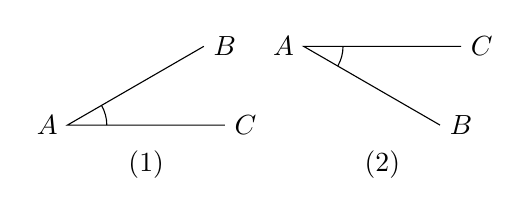
\begin{tikzpicture}[>=latex, scale=1]
\begin{scope}
\draw(30:2)node[right]{$B$}--(0,0)node[left]{$A$}--(2,0)node[right]{$C$};
\node at (1,-.5){(1)};
\draw(0.5,0) arc (0:30:.5);
\end{scope}
\begin{scope}[xshift=3cm]
    \draw(2,1)node[right]{$C$}--(0,1)node[left]{$A$}--+(-30:2)node[right]{$B$};
    \node at (1,-.5){(2)};
    \draw(0.5,1) arc (0:-30:.5);
\end{scope}
    \end{tikzpicture}
    \caption{}
    \end{minipage}
    \end{figure}

\begin{rmk}
    如图6.18(1)连结测点$A$和目的物$B$, 并且经过$A$点画和
$AB$在同一铅直平面内的水平线$AC$, 如$AB$在$AC$的上方,那么
$\angle BAC$叫做仰角;如图6.18(2), 如果$AB$在$AC$的下方,那么
$\angle CAB$叫做俯角。
\end{rmk}  


\begin{example}
    如图6.19, 已知$C$、$D$两点与物体“$\overline{AB}$”的底端$B$
点共线,且
$\overline{CD}=a$, 仪器$\overline{CC'}$、$\overline{DD'}$的高都等于$b$, 在$C'$、
$D'$两点测得物体的顶端$A$的仰角分别是$\alpha$、$\beta$, 求物体的高
$\overline{AB}$
\end{example}

\begin{figure}[htp]\centering
    \begin{minipage}[t]{0.48\textwidth}
    \centering
    \includegraphics[scale=.5]{fig/6-19.png}
    \caption{}
    \end{minipage}
    \begin{minipage}[t]{0.48\textwidth}
    \centering
    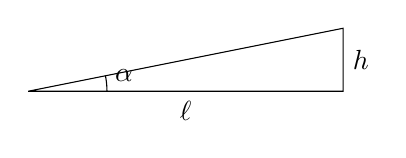
\begin{tikzpicture}[>=latex, scale=1]
\draw(0,0)--node[below]{$\ell$}(4,0)--node[right]{$h$}(4,.8)--(0,0);
\draw(1,0) arc (0:11.3:1)node[right]{$\alpha$};
    \end{tikzpicture}
    \caption{}
    \end{minipage}
    \end{figure}


\begin{solution}
    在直角$\triangle AEC'$与直角$\triangle AED'$中,
\begin{align}
    \overline{C'E}&=\overline{AE}\x \cot\alpha\\
    \overline{D'E}&=\overline{AE}\x \cot\beta
\end{align}
$(6.1)-(6.2)$得:
\[\overline{D'E}-\overline{C'E}=\overline{AE} \x(\cot\beta-\cot\alpha)\]
即:$\overline{C'D'}=\overline{AE} \x(\cot\beta-\cot\alpha)$

已知$\overline{C'D'}=\overline{CD}=a$

$\therefore\quad \overline{AE}=\frac{a}{\cot\beta-\cot\alpha}$

但$\overline{AB}=\overline{AE}+\overline{EB}=\overline{AE} +b$, 

$\therefore\quad \overline{AB}=b+\frac{a}{\cot\beta-\cot\alpha}$

\end{solution}

如果要测底部可以到达的物体的高度,可用例6.22所介绍
的方法,如要测底部不能到达的的物体的高度,可用例6.23所
介绍的方法。

\begin{example}
    一条公路的路面升高$h$与水平距离$\ell$的比值$i$叫做
    路面的坡度。即$i=h:\ell$ (图6.20). 已知某段公路,每前进
    100米就升高4米,求路面的坡度及路面对水平面的倾角$\alpha$.
\end{example}

\begin{solution}
    路面的坡度$i=\frac{h}{\ell}$
    ,已知$h=4$米,$\ell=100$米,

$\therefore\quad  i=\frac{4}{100}=0.04$

    从图6.20中的直角三角形可
    见,$h:\ell$正好是角$\alpha$的正切,即:$i=\tan\alpha$,
    
    $\therefore\quad \tan\alpha=0.04$. 倒查正切表得:
    $\alpha=2^{\circ}17'$.

    答:路面的坡度是0.04, 路面对水平面的倾角是$2^{\circ}17'$.
\end{solution}

\begin{example}
   已知一门式起重
机(图6.21),机身高21
米,吊杆长$\overline{AB}=36$米,吊
杆的倾角$A$(即吊杆与水平
线的夹角)可以从$30^{\circ}$转到
$80^{\circ}$, 求这门起重机工作时
的最大高度和最大水平距
离。
\end{example}
    
\begin{figure}[htp]
    \centering
\includegraphics[scale=.6]{fig/6-21.png}
    \caption{}
\end{figure}

\begin{solution}
    当吊杆$\overline{AB}$的倾角
    $A$达到最大限度$80^{\circ}$时,这时
    起重机吊的最高位置如图6.
    21中$\overline{AB}$的位置.在直角
    $\triangle ABC$中,$\angle A=80^{\circ}$, 
   $\overline{AB}=36$米,因此:
\[    \overline{EC}=\overline{AB} \x \sin80^{\circ}=36\x\sin80^{\circ}
    =36\x0.9848\approx 35.45{\rm m}\]
\[\text{起重机的最大高度}=\text{机身高}+\overline{BC}=21+35.45=56.45{\rm m}\]

当倾角$A$达到最小角时,起吊的水平距离最远,这时,
如图6.21中$\overline{AB'}$的位置。在直角$\triangle AB'C'$中,$\angle A=30^{\circ}$, 
$\overline{AB'}=36$米。

因此:起重机起吊的最远水平距离
\[\overline{AC'}=\overline{AB'}\x\cos30^{\circ}=36\x0.8660
\approx 31.18{\rm m}\]

答:起重机工作的最大高度是56.45米,最远水平距离
是31.18米。
\end{solution}

\begin{ex}
\begin{enumerate}
    \item 测量学校旗杆的高度。
    \item 选择底部不能到达的建筑物或树本,测量它的高度。
    \item 如图,要求河两岸$B$、$C$两点间的距离,在$B$点这一岸垂
    直于$BC$方向上找一点$A$, 测出$\angle BAC=58^{\circ}12'$,
    $\overline{AB}=25$米,求$B$、$C$两点间的距离。
    \item 如图,从山顶$D$测得地平面上同一方向的两点$A$和$B$的俯
角分别是$18^{\circ}$和$23^{\circ}$, 已知$\overline{AB}=140$米,求山高
$\overline{CD}$(得数保留整数米)。
\item 已知传送带和地面的夹角是$25^{\circ}$, 它把物件从地面运到
离地面9米高的地方,求物件所走的路程。
\item 工件上有V形槽,测出上口宽200mm,深19.2mm,
求V形角$\alpha$多大。
\item 如图,在离地面高5米处引拉线固定电线杆,拉线和地
面成$60^{\circ}$角,求每根拉线多长,拉线底端离杆底多远。
\end{enumerate}
\end{ex}

\begin{figure}[htp]\centering
    \begin{minipage}[t]{0.3\textwidth}
    \centering
\includegraphics[scale=.7]{fig/6-3ti.PNG}
    \caption*{第3题}
    \end{minipage}
    \begin{minipage}[t]{0.6\textwidth}
    \centering
    \includegraphics[scale=.7]{fig/6-4ti.PNG}
    \caption*{第4题}
    \end{minipage}
    \end{figure}

\begin{figure}[htp]\centering
    \begin{minipage}[t]{0.48\textwidth}
    \centering
\begin{tikzpicture}[>=latex, scale=1]
\tkzDefPoints{0/0/A, 4/0/B, 4/2/C, 2.7/2/D, 2/1/E, 1.3/2/F, 0/2/G}
\tkzDrawPolygon(A,B,C,D,E,F,G)
\draw[dashed](F)--node[above]{20}(D);
\draw[<->](3.5,1)--node[fill=white]{19.2}(3.5,2);
\draw(E)--(3.7,1);
\tkzMarkAngle[mark=none, size=.3](D,E,F)
\node at (E)[above=.2]{$\alpha$};
    \end{tikzpicture}
    \caption*{第6题}
    \end{minipage}
    \begin{minipage}[t]{0.48\textwidth}
    \centering
    \begin{tikzpicture}[>=latex, scale=1]
\fill[pattern=north east lines](-2,-.25) rectangle (2.5,0);
\draw(-2,0)--(2.5,0);
\draw[very thick](-1.75,0)--(0,3.03)--(1.75,0);
\draw(-.04,0) rectangle (.04,3.5);
\draw(0,3.03)--(2.5,3.03);
\draw[<->](2.25,0)--node[fill=white]{5m}(2.25,3.03);
\draw(-1.25,0) arc (0:60:.5)node[right]{$60^{\circ}$};
    \end{tikzpicture}
    \caption*{第7题}
    \end{minipage}
    \end{figure}

\subsection*{习题6.2}
\begin{enumerate}
    \item 已知等腰$\triangle ABC$, 腰长为5cm, 底边长为8cm, 求
    $\angle A$、$\angle B$、$\angle C$.
    \item 把2米的竹杆,垂直于地面的时候,影长1.6米,这时
    太阳的仰角大约是多少度?
    \item  已知等腰$\triangle ABC$, 腰长$\overline{AB}=\overline{AC}=10$cm, 底角为$40^{\circ}$, 
    求高$\overline{AD}$, 底边$\overline{BC}$和面积$S$.
    \item 在$\triangle ABC$中,$\angle B$、
    $\angle C$是锐角,$\overline{AB}=c$, $\overline{AC}=b$, $\overline{AD}$是
    $\overline{BC}$边上的高,求证:
\begin{enumerate}
    \item $\overline{AD}=b\sin C=c\sin B$
    \item $\frac{b}{\sin B}=\frac{c}{\sin C}$
\end{enumerate}
\item 已知正$n$边形的半径是$r$,周长是$\ell$,求证:
\[\ell=2nr\sin\frac{180^{\circ}}{n}\]
\item  一架战斗机从3300米高空以每秒150米的速度向轰炸目
标俯冲,俯冲角为$42^{\circ}$, 在离地面1300米时投弹,击中
目标,问飞机开始俯冲到投弹共用几秒钟?
\begin{figure}[htp]\centering
    \begin{minipage}[t]{0.48\textwidth}
    \centering
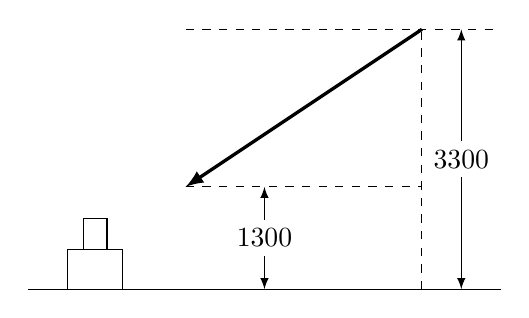
\begin{tikzpicture}[>=latex, scale=1]
\draw(-2,0)--(4,0);
\draw(-1.5,0) rectangle (-.8,.5);
\draw(-1.3,.5) rectangle (-1,.9);
\draw[dashed](0,3.3)--(4,3.3);
\draw[dashed](0,1.3)--(3,1.3);
\draw[dashed](3,0)--(3,3.3);
\draw[very thick, ->](3,3.3)--(0,1.3);
\draw[<->] (3.5,3.3)--node[fill=white]{3300}(3.5,0);
\draw[<->] (1,1.3)--node[fill=white]{1300}(1,0);
    \end{tikzpicture}
    \caption*{第6题}
    \end{minipage}
    \begin{minipage}[t]{0.48\textwidth}
    \centering
    \begin{tikzpicture}[>=latex, scale=.8]
\draw(0,0)node[left]{$A$}--node[above]{2km}(4,0)node[right]{$B$};
\draw[dashed](0,-2)--(0,0)--(4,-4.767)node[below]{$C$}--(4,0);
\draw(0,-.5) arc (-90:-50:.5)node[below=4pt]{$40^{\circ}$};
    \end{tikzpicture}
    \caption*{第7题}
    \end{minipage}
    \end{figure}

\item 东西两炮台$A$、$B$相距2km, 同时发现入侵敌舰$C$, 炮台
$A$测得敌舰$C$在它的南偏东$40^{\circ}$的方向,炮台$B$测得敌舰$C$
在它的正南方,试求敌舰与两炮台的距离。

\item 
从圆外一点向圆引两条切线,已知切线长等于21.8cm, 
圆的半径等于10.6cm, 求这两条切线间的夹角。
\end{enumerate}

\section{任意三角形中的边角关系}
\subsection{正弦定理}

为了解任意的三角形,下面我们用三角比来研究任意三
角形中的边角关系。

我们约定在$\triangle ABC$中,$\angle A$、$\angle B$、$\angle C$分别用$\alpha$、$\beta$、$\gamma$
来表示;$\angle A$、$\angle B$、$\angle C$的对边分别用$a$、$b$、$c$来表示;外
接圆的半径用$r$来表示。

假定$\alpha$是锐角(图6.22),作$\triangle ABC$的外接圆$O$, 再作$\odot O$的直径$\overline{CA'}$, 弦$\overline{BA'}$, 在$\triangle A'BC$中,$\angle A'BC$是直角,因此$a=2r\sin A'$

$\because\quad \angle A'=\angle A=\alpha$

$\therefore\quad a=2r\sin\alpha$,因此:
\begin{equation}
\frac{a}{\sin\alpha}=r
\end{equation}

\begin{figure}[htp]\centering
    \begin{minipage}[t]{0.48\textwidth}
    \centering
\begin{tikzpicture}[>=latex, scale=1]
\draw[thick](0,0) circle(2);
\tkzDefPoints{0/0/O}
\tkzDefPoint(40:2){B}\tkzDefPoint(-30:2){C}\tkzDefPoint(-170:2){A}\tkzDefPoint(150:2){A'}
\tkzDrawPolygon(A,B,C)
\tkzDrawPolygon[dashed](A',B,C)
\tkzAutoLabelPoints[center=O](A,B,C,A')
\tkzLabelPoints[right](O)
\tkzDrawPoints(O)
\tkzMarkAngles[mark=none, size=.5](C,A,B C,A',B)
\node at (5:2)[left]{$a$};

    \end{tikzpicture}
    \caption{}
    \end{minipage}
    \begin{minipage}[t]{0.48\textwidth}
    \centering
    \begin{tikzpicture}[>=latex, scale=1]
  \draw[thick](0,0) circle(2);
\tkzDefPoint(120:2){B}\tkzDefPoint(-120:2){C}\tkzDefPoint(180:2){A}\tkzDefPoint(60:2){A'}    
\tkzLabelPoints[right](O)
\tkzDrawPoints(O)
\tkzDefPoints{0/0/O}
\tkzDrawPolygon(A,B,C)
\tkzDrawPolygon[dashed](A',B,C)
\tkzAutoLabelPoints[center=O](A,B,C,A')
\tkzMarkAngles[mark=none, size=.4](C,A,B B,A',C)

    \end{tikzpicture}
    \caption{}
    \end{minipage}
    \end{figure}

假定$\angle A$是钝角(图6.23),作$\triangle ABC$的外接圆$\odot O$, 再
作直径$\overline{CA'}$, 弦$\overline{BA'}$

$\because\quad \angle A+\angle A'=180^{\circ}$

$\therefore\quad \angle A'=180^{\circ}-\angle A$, $\angle A'$是一个锐角,

在直角$\triangle A'BC$中,$\angle A'BC$是直角。

$\therefore\quad a=2r\sin A'=2r\sin(180^{\circ}-A)=2r\sin(180^{\circ}-\alpha)$,因此:
\begin{equation}
    \frac{a}{\sin(180^{\circ}-\alpha)}=2r
\end{equation}

我们比较(6.3)、(6.4)两式,可以
看出,如果我们定义一个钝角的正弦
等于它的补角的正弦,即
\[\sin\alpha  =\sin(180^{\circ}-\alpha )\]
其中:$\alpha$ 是钝角。
那么(6.4)式在形式上就与(6.3)式相同
了,这就是说,$\alpha$ 不论是锐角还是钝角
都有:
\[\frac{a}{\sin\alpha}=2r\]

\begin{figure}[htp]
    \centering
\begin{tikzpicture}
    \draw[thick](0,0) circle(2);
    \tkzDefPoint(100:2){B}\tkzDefPoint(-80:2){C}\tkzDefPoint(-130:2){A}
    \tkzDefPoints{0/0/O}
    \tkzLabelPoints[right](O)    \tkzDrawPoints(O)
    \tkzDrawPolygon(A,B,C)
    \tkzAutoLabelPoints[center=O](A,B,C)
    \tkzMarkRightAngle[size=.2](C,A,B)
\end{tikzpicture}
    \caption{}
\end{figure}

当$\alpha$是直角时(图6.24),作直角$\triangle ABC$的外接圆$\odot O$
这时斜边$\alpha$正好是$O$的直径。

$\because\quad \sin90^{\circ}=1$

$\therefore\quad \frac{a}{\sin\alpha}=2r$
仍然成立。

同理,我们还可得出,
\[\frac{b}{\sin\beta}=2r,\qquad \frac{c}{\sin\gamma}=2r\]

总结上面的讨论,我们得到:

\begin{blk}
    {正弦定理}
在任意$\triangle ABC$中,边角关系满足:
\[\frac{a}{\sin\alpha}=\frac{b}{\sin\beta}=\frac{c}{\sin\gamma}=2r\]
\end{blk}

\begin{example}
    已知等边$\triangle ABC$的边长是$a$, 求$r$。
\end{example}

\begin{solution}
$\because\quad \frac{a}{\sin\alpha}=2r,\quad \alpha=60^{\circ}$

$\therefore\quad \frac{a}{\sin60^{\circ}}=2r$
\[r=\frac{a}{2\sin60^{\circ}}=\frac{a}{2\cdot \frac{\sqrt{3}}{2}}=\frac{\sqrt{3}}{3}a\]
\end{solution}

\begin{example}
    在$\triangle ABC$中,已知$b\sin\beta=c\sin\gamma$, 求证$\triangle ABC$是等腰三角形。
\end{example}   

\begin{proof}
$\because\quad b\sin\beta=c\sin\gamma$

$\therefore\quad \frac{b}{c}=\frac{\sin\gamma}{\sin\beta}$

又$\because\quad \frac{b}{\sin\beta}=\frac{c}{\sin\gamma}$

$\therefore\quad \frac{c}{b}=\frac{\sin\gamma}{\sin\beta},\quad \frac{b}{c}=\frac{c}{b},\quad b^2=c^2$

$\because\quad b>0,\quad c>0$

$\therefore\quad b=c$,$\triangle ABC$是等腰三角形。
\end{proof}

\begin{example}
    已知$P$点是$\triangle ABC$的$\overline{BC}$边上的任一点,求证:
\[\frac{\overline{BP}}{\overline{PC}}=\frac{c\sin \angle PAB}{b\sin\angle PAC}\]
\end{example}

\begin{proof}
    如图6.25所示,在$\triangle ABP$与$\triangle APC$中,根据正弦
    定理有:
\[\frac{\overline{BP}}{\sin \angle PAB}=\frac{c}{\sin \angle APB},\qquad \frac{\overline{PC}}{\sin \angle PAC}=\frac{b}{\sin\angle APC}\]
即:    
\[\overline{BP}=\frac{c\sin \angle PAB}{\sin \angle APB},\qquad \overline{PC}=\frac{b\sin \angle PAC}{\sin \angle APC}\]

$\because\quad \angle APB+\angle APC=\pi$    

$\therefore\quad \sin \angle APB=\sin\angle APC,\qquad \frac{\overline{BP}}{\overline{PC}}=\frac{c\sin\angle PAB}{b\sin\angle PAC}$
\end{proof}

\begin{figure}[htp]
    \centering
\begin{tikzpicture}[scale=.8]
\tkzDefPoints{0/0/B, 5/0/C, 2/3/A, 1.5/0/P}
\tkzDrawPolygon(A,B,C)
\tkzDrawSegments(A,P)
\tkzLabelPoints[above](A)
\tkzLabelPoints[below](B,C,P)
\node at (1,1.5)[left]{$c$};
\node at (3.5,1.5)[right]{$b$};
\end{tikzpicture}
    \caption{}
\end{figure}

\begin{ex}
\begin{enumerate}
    \item 求证在$\triangle ABC$中,
\begin{enumerate}
    \item $\sin\alpha=\frac{a}{b}\sin\beta=\frac{a}{c}\sin\gamma$
    \item $a+b+c=2r(\sin\alpha +\sin\beta+\sin\gamma)$
    \item $\sin\alpha+\sin\beta<\sin\gamma$
\end{enumerate}

\item 在$\odot O$中,量得一个$30^{\circ}$的圆周角所对的弦长是4cm,
求$\odot O$的半径$r$.
\item 求下列各角的正弦:
\[90^{\circ},\quad 120^{\circ},\quad 150^{\circ},\quad 135^{\circ},\quad 132^{\circ}\]
\item 在半径是5cm的圆中,$120^{\circ}$的圆心角所对的弦长是多
少?
\item 在半径是15cm的圆中,一条长18cm的弦所对的圆心角
是多少度(精确到度)。
\item 应用正弦定理证明三角形内角平分线定理(提示:模仿
例6.28的证法)。
\end{enumerate}
\end{ex}

\subsection{余弦定理}
在$\triangle ABC$中,如果$\beta$、$\gamma$都是锐角(图6.26),作$\overline{BC}$边
上的高$\overline{AD}$, 则$a=\overline{BD}+\overline{DC}$.

但$\overline{BD}=c\cos\beta$, $\overline{DC}=b\cos\gamma$,因此:
\begin{equation}
    a=c\cos\beta+b\cos\gamma
\end{equation}

如果$\beta$、$\gamma$中有一个是钝角,设$\gamma$是钝角(图6.27)作
$\overline{BC}$边上的高$\overline{AD}$, 这时垂足$D$落在$\overline{BC}$的延长线上,则$a=\overline{BD}-\overline{CD}$。但$\overline{BD}=c\cos\beta$, $\overline{CD}=b\cos(180^{\circ}-\gamma)$,因此:
\begin{equation}
    a=c\cos\beta -b\cos(180^{\circ}-\gamma)
\end{equation}

比较(6.5)、(6.6)两式,为了使它们在形式上得到一致,
我们定义钝角Y的余弦为:
\[\cos\gamma=-\cos(180^{\circ}-\gamma)\qquad \text{($\gamma$为钝角)}\]
这样,不论$\gamma$是锐角还是钝角都有关系式
\[a=c\cos\beta +b\cos\gamma\]
如果$\beta$ 是钝角,由$\cos\beta =-\cos(180^{\circ}-\beta )$同样可以得到:
\[a=c\cos\beta +b\cos\gamma\]

\begin{figure}[htp]\centering
    \begin{minipage}[t]{0.32\textwidth}
    \centering
\begin{tikzpicture}[>=latex, scale=1]
\tkzDefPoints{0/0/B, 3/0/C, 2/2/A, 2/0/D}
\tkzLabelPoints[below](B,C,D)
\tkzLabelPoints[above](A)   
\tkzDrawPolygon(A,B,C)
\node at (1,1)[left]{$c$};  \node at (2.5,1)[right]{$b$};
\node at (1,0)[below]{$a$};  \draw(A)--(D);
\tkzMarkRightAngle[size=.2](A,D,B)
\tkzMarkAngles[size=.3, mark=none](A,C,D C,B,A)
\tkzLabelAngle[pos=.5pt](A,C,D){$\gamma$}
\tkzLabelAngle[pos=.5pt](C,B,A){$\beta$}

    \end{tikzpicture}
    \caption{}
    \end{minipage}
    \begin{minipage}[t]{0.32\textwidth}
    \centering
\begin{tikzpicture}[>=latex, scale=1]
    \tkzDefPoints{0/0/B, 2/0/C, 3/2/A, 3/0/D}     
    \tkzLabelPoints[below](B,C,D)
\tkzLabelPoints[above](A)   
\tkzDrawPolygon(A,B,C)
\draw[dashed](A)--(D)--(C);
\tkzMarkRightAngle[size=.2](A,D,B)
\node at (1.5,1)[left]{$c$};  \node at (2.5,1)[right]{$b$};
\node at (1,0)[below]{$a$};  
\tkzMarkAngles[size=.3, mark=none](A,C,B)
\tkzLabelAngle[pos=.5pt](A,C,B){$\gamma$}
    \end{tikzpicture}
    \caption{}
    \end{minipage}
    \begin{minipage}[t]{0.32\textwidth}
    \centering
    \begin{tikzpicture}[>=latex, scale=1]
\tkzDefPoints{0/0/B, 2/0/C, 2/2.5/A}
\tkzDrawPolygon(A,B,C)
\tkzLabelPoints[below](B,C)
\tkzLabelPoints[above](A)   
\tkzMarkRightAngle[size=.2](A,C,B)

    \end{tikzpicture}
    \caption{}
    \end{minipage}
    \end{figure}


如果$\beta$、$\gamma$中有一个是直角,设$\gamma=90^{\circ}$ (图6.28), 

$\because\quad \cos\gamma=\cos90^{\circ}=0$

$\therefore\quad a=c\cos\beta +b\cos\gamma$ 仍然成立。

若分别作$\overline{AB}$、$\overline{AC}$边上的高,同样还可证明
\[\begin{split}
  b&=a\cos\gamma+c\cos\alpha \\
c&=b\cos\alpha+a\cos\beta  
\end{split}\]

总结上面的讨论,我们得到:

\begin{blk}
 {定理}
在任意$\triangle ABC$中,边角关系满足:
\begin{align}
 a&=c\cos\beta +b\cos\gamma\\
b&=a\cos\gamma+c\cos\alpha \\
c&=b\cos\alpha +a\cos\beta 
\end{align}  
\end{blk}

由上面的定理,我们就可推出余弦定理

\begin{blk}
    {余弦定理}
在任意的$\triangle ABC$中,边角关系满足
\[\begin{split}
  a^2&=b^2+c^2-2bc\cos\alpha\\
b^2&=c^2+a^2-2ca \cos\beta\\
c^2&=a^2+b^2-2ab\cos\gamma  
\end{split}\]
\end{blk}

\begin{proof}
    由上面的定理的(6.7)式得,
\[\cos\beta=\frac{a-b\cos\gamma}{c}\]
由(6.8)式得
\[\cos\alpha=\frac{b-a\cos\gamma}{c}\]
把$\cos\beta$、$\cos\alpha$代入(6.9)得
\[c=a\frac{a-b\cos\gamma}{c}+b\frac{b-a\cos\gamma}{c}=\frac{a^2+b^2-2ab\cos\gamma}{c}\]
$\therefore\quad c^2=a^2+b^2-2ab\cos\gamma$

用同样的办法我们可证:
\[\begin{split}
   b^2&=c^2+a^2-2ca \cos\beta\\ 
   a^2&=b^2+c^2-2bc\cos\alpha   
\end{split}\]
\end{proof}

请同学们自证如下两个推论:

\begin{blk}{推论1}
在$\triangle ABC$中,
\[\begin{split}
    \cos\alpha&=\frac{b^2+c^2-a^2}{2bc}\\
    \cos\beta&=\frac{a^2+c^2-b^2}{2ac}\\
        \cos\gamma&=\frac{a^2+b^2-c^2}{2ab}
\end{split}\]
\end{blk}

\begin{blk}{推论2}
     一个三角形两边平方的和如果等于第三边的平
方,那么第三边所对的角是直角;如果小于第三边的平方,
那么第三边所对的角是钝角;如果大于第三边的平方,那么
第三边所对的角是锐角。
\end{blk}


\begin{example}
    分别求出$120^{\circ}$、$135^{\circ}$、$150^{\circ}$、$140^{\circ}$的余弦。
\end{example}

\begin{solution}
由定义知,一个钝角的余弦等于它的补角的余弦的
相反数,所以有:
\[\begin{split}
  \cos120^{\circ}&=-\cos(180^{\circ}-120^{\circ})=-\cos60^{\circ}=-\frac{1}{2}\\
  \cos135^{\circ}&=-\cos(180^{\circ}-135^{\circ})=-\cos45^{\circ}=-\frac{\sqrt{2}}{2}\\  
  \cos150^{\circ}&=-\cos(180^{\circ}-150^{\circ})=-\cos30^{\circ}=-
\frac{\sqrt{3}}{2}\\
\cos140^{\circ}&=-\cos(180^{\circ}-140^{\circ})=-\cos40^{\circ}\approx -0.7660  
\end{split}\]
\end{solution}

\begin{example}
    用余弦定理证明广义勾股定理。

    已知:$\parallelogram ABCD$ (图6.29)

    求证:
    $\overline{AC}^2+\overline{BD}^2=2(\overline{AB}^2+\overline{AD}^2)$
\end{example}

\begin{figure}[htp]
    \centering
\begin{tikzpicture}
 \tkzDefPoints{0/0/A, 3/0/B, 3.75/1.5/C, .75/1.5/D}
\tkzDrawPolygon[thick](A,B,C,D)
\tkzDrawSegments[thick](A,C B,D)
\tkzLabelPoints[below](A,B)
\tkzLabelPoints[above](C,D)   
\end{tikzpicture}
    \caption{}
\end{figure}

\begin{proof}
在$\triangle ABC$与$\triangle ABD$中,
\begin{align}
   \overline{AC}^2&=\overline{AB}^2+\overline{BC}^2-2\overline{AB}\cdot \overline{BC} \cos\angle ABC \\
    \overline{BD}^2&=\overline{AB}^2+\overline{AD}^2-2\overline{AB}\cdot \overline{AD}\cos\angle BAD
\end{align}

$\because\quad \angle BAD+\angle ABC =180^{\circ}$

$\therefore\quad \cos \angle ABC=-\cos\angle BAD$

又$\because\quad \overline{BC}=\overline{AD}$

$(6.10)+(6.11)$则得:
\[\overline{AC}^2+\overline{BD}^2=\overline{AB}^2+\overline{BC}^2+\overline{AB}^2+\overline{AD}^2=2\left(\overline{AB}^2+\overline{AD}^2\right)\]
\end{proof}

\begin{ex}
\begin{enumerate}
    \item 在$\triangle ABC$中,已知$a=4$, $b=7$, $\gamma=40^{\circ}$, 求$c$.
    \item 在$\triangle ABC$中,已知$a=2$, $b=3$, $c=4$, 求$\cos\alpha$、$\cos\beta$、
    $\cos\gamma$.
    \item 已知$\triangle ABC$的三边:
\begin{enumerate}
    \item 56, 65, 33, 求最大角;
    \item 7、$4\sqrt{3}$、$\sqrt{13}$, 求最小角。
\end{enumerate}

    \item 在$\triangle ABC$中,$\angle A=120^{\circ}$, 求证:
\begin{enumerate}
    \item $a^2-b^2=c(b+c)$
    \item $ b(a^2-b^2)=c(a^2-c^2)$
\end{enumerate}

\item  在$\triangle ABC$中,已知$\cos\beta=\frac{\sin\alpha}{2\sin\gamma}$, 求证$\triangle ABC$是等腰三角形。
\item  在$\triangle ABC$中,求证:
\[\frac{\cos A}{a}+\frac{\cos B}{b}+\frac{\cos C}{c}=\frac{a^2+b^2+c^2}{2abc}\]
\end{enumerate}    
\end{ex}

\subsection{解斜三角形}
在一个三角形中,如果没有一个角是直角,那么,这个三角
形叫做斜三角形。斜三角形的解法可以分成下面的四种情形:
\begin{enumerate}
\item 已知一边和两角;
\item 已知两边和它们的夹角;
\item 已知三边;
\item 已知两边和其中一边的对角。
\end{enumerate}

下面我们分别举例说明每种情形的解法。
    
\begin{example}
    已知:$c=100$、$\alpha=40^{\circ}$, $\beta=60^{\circ}$ (图6.30), 求
$\gamma$、$a$、$b$.
\end{example}

\begin{figure}[htp]
    \centering
\begin{tikzpicture}
\tkzDefPoints{0/0/A, 4/0/B, 2.8/2/C}
\tkzDrawPolygon(A,B,C)
\tkzMarkAngles[mark=none, size=.3](B,A,C C,B,A)
\tkzLabelPoints[below](A,B)
\tkzLabelPoints[above](C)
\end{tikzpicture}
    \caption{}
\end{figure}

\begin{solution}
\[\begin{split}
    \gamma&=180^{\circ}-(40^{\circ}+60^{\circ})=80^{\circ}\\
    a&=\frac{c\sin\alpha}{\sin\gamma}\approx \frac{100\x \sin 40^{\circ}}{\sin 80^{\circ}}=\frac{100\x 0.6428}{0.9848}=65.27\\
    b&=\frac{c\sin\beta}{\sin\gamma}=\frac{100\x \sin 60^{\circ}}{\sin 80^{\circ}}=\frac{100\x 0.8660}{0.9848}=87.94
\end{split}\]
\end{solution}

例6.31告诉我们,如果已知两角和一边,先用内角和定理
求出未知的第三个角,然后再用正弦定理便可求出未知的两
边了。

\begin{ex}
\begin{enumerate}
    \item 已知下列条件,解三角形,并求其外接圆的半径。
\begin{enumerate}
    \item $b=4,\qquad \alpha=30^{\circ} ,\qquad \beta=120^{\circ} $
    \item $c=13,\qquad \alpha=45^{\circ},\qquad \beta=60^{\circ} $
\end{enumerate}
    \item 解三角形:
\begin{enumerate}
    \item $\alpha=62^{\circ} ,\qquad \beta=48^{\circ} ,\qquad c=24$
    \item $\alpha=55^{\circ} 12',\qquad \beta=29^{\circ} 18',\qquad c=18$
\end{enumerate}
\end{enumerate}
\end{ex}


\begin{example}
    已知$b=60$、$c=34$、$\alpha=41^{\circ}$ (图6.31)。求$\alpha$, $\beta$,
$\gamma$.
\end{example}

\begin{figure}[htp]
    \centering
\begin{tikzpicture}
\tkzDefPoints{0/0/B, 4/0/C, 1.5/2/A}
\tkzDrawPolygon(A,B,C)
\tkzMarkAngles[mark=none, size=.3](B,A,C)
\tkzLabelPoints[below](C,B)
\tkzLabelPoints[above](A)
\node at (2,0)[below]{$a$};
\node at (5.5/2,1)[right]{$b$};
\node at (.75,1)[left]{$c$};
\end{tikzpicture}
    \caption{}
\end{figure}

\begin{solution}
\[\begin{split}
    a^2&=b^2+c^2-2bc\cos\alpha\\
&=602+342-2\x60\x34\cos41^{\circ}\\
&=3600+1156-4080\x0.755\approx 1676
\end{split}\]
查平方根表,得:$a\approx 41$。
\[\sin\gamma=\frac{c\sin\alpha}{a}=\frac{34\x\sin41^{\circ}}{41}=\frac{34\x 0.655}{41}\approx 0.5441\]

$\therefore\quad \gamma\approx 32^{\circ}58'$

\[\beta=180^{\circ}-(\alpha+\gamma)
=180^{\circ}-(41^{\circ}+32^{\circ}58')
=106^{\circ}2'\]    
\end{solution}


例6.32告诉我们,如果已知两边及夹角,可由余弦定理先求
出未知的一边,然后由正弦定理就可算出未知的一个角了,
再由内角和定理,就可求出未知的另一个角了。再求出未知
边后,最好先求较短边所对的角,因为较短边所对的角一定
是锐角,这样就可避免求钝角的情况。

\begin{ex}
    已知下列条件,解三角形
\begin{enumerate}
\item  $a=22,\qquad b=26,\qquad \gamma=78^{\circ}$
\item  $b=10,\qquad c=10,\qquad \alpha=102^{\circ}$
\item  $a=0.8,\qquad c=0.6,\qquad \beta=50^{\circ}$
\item  $a=4,\qquad b=5,\qquad \gamma=60^{\circ}$
\end{enumerate}
\end{ex}

\begin{example}
    已知$a=134.6$, $b=87.8$, $c=161.7$(图6.32),
    求$\alpha$、$\beta$、$\gamma$.
\end{example}

\begin{figure}[htp]
    \centering
\begin{tikzpicture}
    \tkzDefPoints{0/0/C, 3/0/B, 0/2.5/A}
\tkzDrawPolygon(A,B,C)
\tkzLabelPoints[below](B,C)
\tkzLabelPoints[above](A)
\node at (1.5,0)[below]{$a$};
\node at (0,1.25)[left]{$b$};
\node at (1.5,1.25)[right]{$c$};
\end{tikzpicture}
    \caption{}
\end{figure}

\begin{solution}
\textbf{解法一:} 先用余弦定理求两个较短的边所对的角。
\[\cos\alpha=\frac{87.8^2+161.7^2-134.6^2}{2\x 87.8\x 161.7}\approx 0.5549\]
$\therefore\quad \alpha=56^{\circ}18'$

\[\cos\beta=\frac{134.6^2+161.7^2-87.8^2}{2\x134.6\x161.7}\approx 0.8400\]
$\therefore\quad \beta=32^{\circ}51',\quad 
\gamma=180^{\circ}-(56^{\circ}18'+32^{\circ}51')=90^{\circ}51'$

\textbf{解法二:} 
\[\cos\alpha=\frac{87.8^2+161.7^2-134.6^2}{2\x 87.8\x 161.7}\approx 0.5549\]
$\therefore\quad \alpha=56^{\circ}18'$
    
\[\sin\beta=\frac{b}{a}\sin\alpha=\frac{87.8\x \sin 56^{\circ}18'}{134.6}\approx 0.5427\]
$\therefore\quad \beta=32^{\circ}51', \quad \gamma=180^{\circ}-(56^{\circ}18'+32^{\circ}51')=90^{\circ}51'$
\end{solution}

由例6.33可知,如果已知三边$a$、$b$、$c$, 可用余弦定理求
出两个较短的边所对的角的余弦;或由余弦定理求出一角
后,再改用正弦定理求另一角的正弦。一般地说后一种方法
比较方便。我们所以要先求较短边所对的角,主要还是避免
在计算中出现求钝角的情况。

\begin{ex}
    已知下列条件,解三角形
\begin{enumerate}
\item $a=40,\qquad b=19,\qquad c=41$
\item $a=1.5,\qquad b=2.5,\qquad c=1.8$
\item $a=6,\qquad b=3,\qquad c=3\sqrt{3}$
\item $a=\sqrt{10},\qquad b=4,\qquad c=\sqrt{2}$   
\end{enumerate}
\end{ex}

\begin{example}
    在锐角$\triangle ABC$中,已知$a=12$, $b=20$, $\alpha=34^{\circ}$, 
    求:$\beta$、$\gamma$和$c$ (图6.33).
\end{example}

\begin{figure}[htp]
    \centering
\begin{tikzpicture}
\tkzDefPoints{0/0/A, 4/0/B, 3.2/2.5/C, 2.4/0/B'}
\tkzDrawPolygon(A,B,C)
\tkzLabelPoints[below](A,B,B')
\tkzLabelPoints[above](C)
\tkzDrawSegments[dashed](C,B')
\node at (1.6,1.25)[left]{$b$};
\node at (3.6,1.25)[right]{$a$};
\tkzDrawArc[delta=10](C,B')(B)
\end{tikzpicture}
    \caption{}
\end{figure}


\begin{solution}
$\because\quad \frac{a}{\sin\alpha}=\frac{b}{\sin\beta}$

$\therefore\quad \sin\beta=\frac{b\sin\alpha}{a}=\frac{20\x \sin 34^{\circ}}{12}=\frac{20\x 0.5592}{12}=0.9320$

由于$\beta$是锐角,反查正弦表得:$\beta=68^{\circ}45'$

$\therefore\quad \gamma=180^{\circ}-(\alpha+\beta)=180^{\circ}-(34^{\circ}+68^{\circ}45')=77^{\circ}15'$

又$\because\quad \frac{c}{\sin\gamma}=\frac{a}{\sin\alpha}$

$\therefore\quad c=\frac{a\sin\gamma}{\sin\alpha}=\frac{12\x \sin 77^{\circ}15'}{\sin 34^{\circ}}=\frac{12\x 0.9753}{0.5582}=20.93$
\end{solution}

如果在例6.34中,不限$\triangle ABC$是锐角三角形,那么$\beta$角就
可能是钝角(图6.33中的$\angle AB'C$),这样$\beta$角就有两个解。
对于已知$a$、$b$、$\alpha$解三角形这种情形,我们详细讨论如下:
\begin{enumerate}


\item 如果已知$\alpha$角是钝角或直角,那么必须$a>b$才能有
解(为什么?),这时从$\sin\beta=\frac{b\sin\alpha}{a}$
求$\beta$角的时候,只能
取锐角的值,因此只有一个解。
\item 如果已知的$\alpha$角是锐角,并且$a>b$或者$a=b$. 这时
从$\sin\beta=\frac{b\sin\alpha}{a}$
求$\beta$角的时候,也只能取锐角的值,因此都
只有一个解(图6.34和图6.35)。

\begin{figure}[htp]\centering
    \begin{minipage}[t]{0.48\textwidth}
    \centering
\begin{tikzpicture}[>=latex, scale=1]
\tkzDefPoints{0/0/A, 3/0/B, 1/2/C}
\tkzLabelPoints[below](A,B)
\tkzLabelPoints[above](C)
\tkzDrawPolygon(A,B,C)
\node at (1.5,0)[below]{$c$};
\node at (2,1)[right]{$a>b$};
\node at (.5,1)[left]{$b$};
\tkzDefPointBy[rotation= center C angle -100](B)
\tkzGetPoint{C'}
\tkzDrawArc[delta=10](C,C')(B)
    \end{tikzpicture}
    \caption{}
    \end{minipage}
    \begin{minipage}[t]{0.48\textwidth}
    \centering
    \begin{tikzpicture}[>=latex, scale=1]
\tkzDefPoints{0/0/A, 3/0/B, 1.5/2/C}
\tkzLabelPoints[below](A,B)
\tkzLabelPoints[above](C)
\tkzDrawPolygon(A,B,C)
\node at (1.5,0)[below]{$c$};
\node at (.75,1)[left]{$b$};
\node at (2.25,1)[right]{$a=b$};
\tkzDrawArc[delta=10](C,A)(B)
    \end{tikzpicture}
    \caption{}
    \end{minipage}
    \end{figure}



\item 如果已知的$\alpha$角是锐角,并且$a<b$,我们再分下
面三种情况来讨论:
\begin{enumerate}
    \item $a>b\sin \alpha$, 这时从$\sin\beta=\frac{b\sin\alpha}{a}$求得 $\sin\beta<1$, 
    $\beta$可以取一个锐角的值和一个钝角的值,因此可以有两个解
    (图6.36)。
\begin{figure}[htp]
    \centering
\begin{tikzpicture}
    \tkzDefPoints{0/0/A, 4/0/B, 3/2.5/C, 2/0/B'}
\tkzLabelPoints[below](A,B,B')
\tkzLabelPoints[above](C)
\draw[dashed](C)--node[fill=white]{$b\sin\alpha$}(3,0);
\tkzDrawPolygon(A,B,C)
\tkzDrawSegments(B',C)
\node at (1.5,1.25)[left]{$b$};
\node at (3.5,1.25)[right]{$\begin{array}{cc}
    a>b\sin\alpha\\
    a<b
\end{array}$};
\tkzDrawArc[delta=10](C,B')(B)
\tkzMarkAngles[size=.35, mark=none](B,A,C C,B',A C,B,A)
\end{tikzpicture}
    \caption{}
\end{figure}

  \item $a=b\sin\alpha$, 这时从$\sin\beta=\frac{b\sin\alpha}{a}$
    求得$\sin\beta=1$, 所以
    $\beta$只能是直角,因此,只有一个解(图6.37)。
\item $a<b\sin\alpha$, 这时从$\sin\beta=\frac{b\sin\alpha}{a}$
    求得$\sin\beta>1$, 但是
    一角的正弦值不能大于1, 因此没有解(图6.38)。
\end{enumerate}
\end{enumerate}

\begin{figure}[htp]\centering
    \begin{minipage}[t]{0.48\textwidth}
    \centering
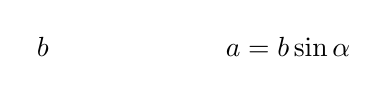
\begin{tikzpicture}[>=latex, scale=1]
\tkzDefPoints{0/0/A, 4/0/B, 4/3/C}
\tkzLabelPoints[below](A,B)
\tkzLabelPoints[above](C)
\node at (2,1.5)[left]{$b$};
\node at (4,1.5)[right]{$a=b\sin\alpha$};
\tkzCompass(C,B)
\tkzDrawPolygon(A,B,C)
    \end{tikzpicture}
    \caption{}
    \end{minipage}
    \begin{minipage}[t]{0.48\textwidth}
    \centering
    \begin{tikzpicture}[>=latex, scale=1]
\tkzDefPoints{0/0/A, 4/0/B, 3/2.5/C, 3.75/.5/D}
\tkzLabelPoints[below](A)
\tkzLabelPoints[above](C)
\draw[dashed](C)--node[fill=white]{$b\sin\alpha$}(3,0);
\node at (3.5,1.5)[right]{$a<b\sin\alpha$};
\tkzCompass[delta=30](C,D)
\tkzDrawSegments(A,C A,B C,D)
    \end{tikzpicture}
    \caption{}
    \end{minipage}
    \end{figure}

上面所得的结果可以列成下表:
\begin{center}
\begin{tabular}{c|c|c}
\hline
& $\alpha\ge 90^{\circ}$ &$\alpha<90^{\circ}$\\
\hline
$a>b$& 一解&一解\\ \hline
$a=b$&无解&一解\\
\hline
& & $a>b\sin\alpha$时,两解\\
$a<b$ &无解 & $a=b\sin\alpha$时,一解\\
& & $a<b\sin\alpha$时,无解\\
\hline
\end{tabular}
\end{center}



\begin{ex}
\begin{enumerate}
\item 已知$a=2,\quad b=3,\quad \alpha=30^{\circ}$, 解三角形。
\item 已知$a=2,\quad b=3,\quad \beta=120^{\circ}$, 解三角形。
\item 已知$b=3,\quad c=4,\quad \beta=45^{\circ}$, 解三角形。
\end{enumerate}   
\end{ex}

\subsection{三角形的面积公式}
在解题中,有时需要根据三角形的已知元素来计算它的
面积,下面导出几个常用的求三角形面积的公式。

\subsubsection{已知三角形的两边及其夹角,求面积}

当已知三角形的两边及其夹角时,它的面积$S_{\triangle}$可表示
成下面的公式:
\[\begin{split}
    S_{\triangle}&=\frac{1}{2} bc\sin\alpha\\
S_{\triangle}&=\frac{1}{2} ac\sin\beta\\
S_{\triangle}&=\frac{1}{2}ab\sin\gamma\\
\end{split}\]

\begin{proof}
\begin{enumerate}
    \item 当$\alpha$、$\beta$都为锐角时
图(6.39),设$\overline{AB}$上的
高$\overline{CD}=h$. 那么,
\[S_{\triangle}=\frac{1}{2}ch\]
在直角$\triangle ACD$中,$h=b\sin\alpha$. 
代入上式得
\[S_{\triangle}=\frac{1}{2}bc\sin\alpha\]

\begin{figure}[htp]\centering
    \begin{minipage}[t]{0.48\textwidth}
    \centering
\begin{tikzpicture}[>=latex, scale=1]
\tkzDefPoints{0/0/A, 4/0/B, 3/2.5/C, 3/0/D}
\tkzLabelPoints[below](A,B,D)
\tkzLabelPoints[above](C)
\tkzDrawPolygon(A,C,B)
\tkzDrawSegments[dashed](C,D)
\tkzMarkAngles[mark=none, size=.35](D,A,C C,B,D)
\tkzLabelAngle[pos=.5](D,A,C){$\alpha$}
\tkzLabelAngle[pos=.5](C,B,D){$\beta$}
\tkzMarkRightAngle(B,D,C)
    \end{tikzpicture}
    \caption{}
    \end{minipage}
    \begin{minipage}[t]{0.48\textwidth}
    \centering
    \begin{tikzpicture}[>=latex, scale=1]
\tkzDefPoints{0/0/D, 4/0/B, 0/2.5/C, 1.3/0/A}
\tkzLabelPoints[below](A,B,D)
\tkzLabelPoints[above](C)
\tkzDrawPolygon(A,C,B)
\tkzDrawSegments[dashed](C,D A,D) 

    \end{tikzpicture}
    \caption{}
    \end{minipage}
    \end{figure}

\item 当$\alpha$为钝角时
(图6.40),仍设$\overline{AB}$边上的高
$\overline{CD}=h$, 那么:
\[S_{\triangle}=\frac{1}{2}ch\]
在直角$\triangle ACD$中,$h=b\sin(180^{\circ}-\alpha)=b\sin\alpha$ 

$\therefore\quad S_{\triangle}=\frac{1}{2}bc\sin\alpha$

当$\beta$为钝角时,同理也可证明:
\[S_{\triangle}=\frac{1}{2}bc\sin\alpha\]
\item 当$\alpha$为直角时,那么,
\[S_{\triangle}=\frac{1}{2}bc \]
但$\sin\alpha=\sin 90^{\circ}=1$

$\therefore\quad S_{\triangle}=\frac{1}{2}bc\sin\alpha$仍然成立。

同理可证:
\[S_{\triangle}=\frac{1}{2} ac\sin\beta,\qquad 
S_{\triangle}=\frac{1}{2}ab\sin\gamma\]
\end{enumerate} 
\end{proof}


\subsubsection{已知三角形的三边求面积}

如果已知三角形的三边,则
\[S_{\triangle}=\sqrt{p(p-a)(p-b)(p-c)} \]
其中:$p=\frac{1}{2}(a+b+c)$

\begin{proof}
    由余弦定理得:
\[\cos\alpha=\frac{b^2+c^2-a^2}{2bc}\]
因此:
\[\begin{split}
    \sin\alpha&=\sqrt{1-\cos^2\alpha}=\sqrt{1-\left(\frac{b^2+c^2-a^2}{2bc}\right)^2}\\
    &=\sqrt{\left(1+\frac{b^2+c^2-a^2}{2bc}\right)\left(1-\frac{b^2+c^2-a^2}{2bc}\right)}\\
    &=\sqrt{\frac{(b+c)^2-a^2}{2bc}\cdot \frac{a^2-(b-c)^2}{2bc}}\\
    &=\frac{1}{2bc}\cdot \sqrt{(b+c+a)(b+c-a)(a+b-c)(a-b+c)}
\end{split}\]

令$p=\frac{1}{2}(a+b+c)$,则$2p=a+b+c$
\[b+c-a=(a+b+c)-2a=2p-2a=2(p-a)\]
同理:
\[a+c-b=2(p-b),\qquad a+b-c=2(p-c)\]
因此:
\[\begin{split}
\sin\alpha&=\frac{1}{2bc}\sqrt{16p(p-a)(p-b)(p-c)}\\
&=\frac{2}{bc}\sqrt{p(p-a)(p-b)(p-c)}
\end{split}\]

由于$S_{\triangle}=\frac{1}{2}bc\sin\alpha$,因此:
\[\begin{split}
    S_{\triangle}&=\frac{1}{2}bc\x \frac{2}{bc}\sqrt{p(p-a)(p-b)(p-c)}\\
    &=\sqrt{p(p-a)(p-b)(p-c)}
\end{split}\]

这个公式,我国叫做\textbf{三斜求积公式},国外又叫做\textbf{海伦公
式}。
\end{proof}

\subsubsection{已知三角形二角一夹边,求三角形的面积}

如果已知三角形的二角一夹边,则
\[\begin{split}
S_{\triangle}&=\frac{a^{2} \sin \beta \cdot \sin \gamma}{2 \sin (\beta+\gamma)} \\
S_{\triangle}&=\frac{b^{2} \sin \alpha \cdot \sin \gamma}{2 \sin (\alpha+\gamma)} \\
S_{\triangle}&=\frac{c^{2} \sin \alpha \cdot \sin \beta}{2 \sin (\alpha+\beta)}
    \end{split}\]

\begin{proof}
已知$S_{\triangle}=\frac{1}{2}bc\sin\alpha$,由正弦正理,
\[b=\frac{a\sin \beta}{\sin\alpha},\qquad c=\frac{a\sin\gamma}{\sin\alpha}\]

因此:
\[S_{\triangle}=\frac{1}{2}\left(\frac{a\sin \beta}{\sin\alpha}\right)\cdot\left(\frac{a\sin\gamma}{\sin\alpha}\right)\cdot \sin\alpha=\frac{a^2\sin\beta\cdot \sin\gamma}{2\sin\alpha}\]
但$\sin\alpha=\sin[180^{\circ}-(\beta+\gamma)]=\sin(\beta+\gamma)$

$\therefore\quad S_{\triangle}=\frac{a^{2} \sin \beta \cdot \sin \gamma}{2 \sin (\beta+\gamma)}$

同理可证明其它两个公式。
\end{proof}


\begin{ex}
\begin{enumerate}
    \item 在三角形中,已知
\begin{enumerate}
\item 两边长分别为4、7, 夹角是$40^{\circ}$,
\item 三边长各为2、4、4.
\item $\alpha=60^{\circ}$、$\beta=80^{\circ}$、$c=12$,
\end{enumerate}
    求它们的面积各等于多少?
    \item 求边长等于$a$的等边三角形的面积。

    \item $r$为$\triangle ABC$的外接圆的半径,求证:
\[S_{\triangle}=2r \sin\alpha\cdot\sin\beta\cdot \sin\gamma\]

\item 已知三角形的三边$a$、$b$、$c$, 且$p=\frac{1}{2}(a+b+c)$, 
求证:内切圆半径
\[r=\sqrt{\frac{(p-a)(p-b)(p-c)}{p}}\]

\item 设$h_a$、$h_b$、$h_c$分别表示$\triangle ABC$的三边$\overline{BC}$、$\overline{CA}$、$\overline{AB}$
上的高,求证:
\[\begin{split}
    h_a&=\frac{2}{a}\sqrt{p(p-a)(p-b)(p-c)}\\
    h_b&=\frac{2}{b}\sqrt{p(p-a)(p-b)(p-c)}\\
    h_c&=\frac{2}{c}\sqrt{p(p-a)(p-b)(p-c)}\\
\end{split}\]
\end{enumerate}
\end{ex}

\subsection{解三角形在测量中的应用}

利用解三角形的原理,可
以解许多实际测量问题。下面
我们来研究如何计算不便测量
的两点间的距离。

测量工作者,为了测量远
方某个目标$C$的距离(图6.41),
总先选定适当长的基线
$\overline{AB}$, 然后从基线两端$A$、$B$, 分别测
得目标$C$的方向与$AB$的夹角为$\alpha$、$\beta$. 那么,根据基线$\overline{AB}$的
长度和$\alpha$、$\beta$的值就可算出$C$点与$A$点、$B$点的距离。以及$C$点
与基线$\overline{AB}$的距离,计算方法如下:

$\because\quad \frac{\overline{AC}}{\sin\beta}=\frac{\overline{AB}}{\sin(\alpha+\beta)},\qquad \frac{\overline{BC}}{\sin\alpha}=\frac{\overline{AB}}{\sin(\alpha+\beta)}$

$\therefore\quad \overline{AC}=\frac{\overline{AB}\sin\beta}{\sin(\alpha+\beta)},\qquad \overline{BC}=\frac{\overline{AB}\sin\alpha}{\sin(\alpha+\beta)}$

设$\overline{CD}$是$\overline{AB}$边上的高且$\overline{CD}=x$, 则$\overline{AD}=x\cot\alpha$, $\overline{BD}=x\cot\beta$
\[\overline{AB}=\overline{AD} +\overline{BD} =x(\cot\alpha +\cot\beta)\]

$\therefore\quad x=\frac{\overline{AB}}{\cot\alpha +\cot\beta}$


\begin{figure}[htp]\centering
    \begin{minipage}[t]{0.4\textwidth}
    \centering
\begin{tikzpicture}[>=latex, scale=1]
    \tkzDefPoints{0/0/A, 4/0/B, 2.5/2.5/C, 2.5/0/D}
    \tkzLabelPoints[below](A,B,D)
    \tkzLabelPoints[above](C)
    \tkzDrawPolygon(A,C,B)
    \tkzDrawSegments(C,D)
    \tkzMarkAngles[mark=none, size=.35](D,A,C C,B,D)
    \tkzLabelAngle[pos=.5](D,A,C){$\alpha$}
    \tkzLabelAngle[pos=.5](C,B,D){$\beta$}
    \tkzMarkRightAngle(B,D,C)
    \node at (1.25,1.25)[left]{$b$};
    \node at (3.25,1.25)[right]{$a$};
    \end{tikzpicture}
    \caption{}
    \end{minipage}
    \begin{minipage}[t]{0.55\textwidth}
    \centering
    \begin{tikzpicture}[>=latex, scale=1]
\draw(0,0) circle (1.5);
\tkzDefPoint(30:1.5){A}
\tkzDefPoint(-30:1.5){B}
\tkzDefPoints{0/0/O, 5/0/C}
\tkzDrawPolygon(A,B,C)
\tkzDrawSegments[dashed](A,O B,O)
\tkzMarkAngles[mark=none, size=.3](B,A,C C,B,A)
\tkzLabelAngle[pos=.6](B,A,C){$\alpha$}
\tkzLabelAngle[pos=.6](C,B,A){$\beta$}
\tkzLabelPoints[above](A)
\tkzLabelPoints[below](B)
    \end{tikzpicture}
    \caption{}
    \end{minipage}
    \end{figure}



在测量中,基线越长,量得越准确,测的精确度就越
高。

天文学家曾用了这个方法测出了地球和月亮间的距离。
1671年两个法国天文学家拉让
德和拉卡伊,一个在柏林,一
个在好望角(这两个城市差不
多位于同一子午线上),测出了
$\alpha$、$\beta$的大小和$AB$的长度(图
6.42)。从而确切地算出了地
月平均距离为385400公里。

在地球上,我们可使用的最长基线是地球的直径,由
于地球绕太阳按椭圆形轨道运行,当我们要测量其它星球到
地球的距离时,可使用的最长基线是地球椭圆轨道的长轴
(图6.43)。

\begin{figure}[htp]
    \centering
\includegraphics[scale=.6]{fig/6-43.png}
    \caption{}
\end{figure}

从以上的分析我们知道,当我们应用解三角形原理在地
球上测量地球与其它星球的距离时,可使用的基线是有限
的,所以星球离地球越远、视角也越小,相对基线就越短,
测的结果也就越不精确了。

\begin{ex}
\begin{enumerate}
    \item 要测量一条河两岸的两点$A$、$B$之间的距离,在$A$点所在
    的岸边选择一条基线$\overline{AC}=380$米,测出
    $\angle BAC=75^{\circ}32'$, $\angle BCA=45^{\circ}35'$, 
    求$A$、$B$间的距离。
    \item 如图,$A$、$B$两地不能直接测量,选同时能看到$A$、$B$的一点
    $C$, 测得$\overline{AC}=280$米,$\overline{BC}=470$米,$\angle ACB=80^{\circ}21'$, 
    求$A$、$B$两地的距离。
    \item 河对岸有两个目标$A$、$B$, 若
    不准过河,如何测量才能
    算出$A$、$B$两点间的距离?
\end{enumerate}
\end{ex}

\begin{figure}[htp]\centering
    \begin{minipage}[t]{0.48\textwidth}
    \centering
    \includegraphics[scale=.7]{fig/6-ti1.PNG}
    \caption*{第1题}
    \end{minipage}
    \begin{minipage}[t]{0.48\textwidth}
    \centering
    \includegraphics[scale=.7]{fig/6-ti2.PNG}
    \caption*{第2题}
    \end{minipage}
    \end{figure}

    \begin{figure}[htp]
        \centering
    \includegraphics[scale=.7]{fig/6-ti3.PNG}
        \caption*{第3题}
    \end{figure}

\subsection*{习题6.3}
\begin{enumerate}
    \item 在$\triangle ABC$中,
\begin{enumerate}
    \item 已知$a=8$、$\beta=40^{\circ}$、$\gamma=90^{\circ}$, 求$b$.
    \item 已知$a=25$、$b=31$、$\gamma=90^{\circ}$, 求$a$、$c$.
    \item 已知$a=6$、$\beta=40^{\circ}$、$\gamma=80^{\circ}$, 求b.
    \item 已知$a=8$、$b=6$、$\alpha=75^{\circ}$, 求$\beta$、$c$.
    \item 已知$a=3$、$b=4$、$c=5$, 求$\gamma$.
\end{enumerate}
\item  已知下列条件,求$S_{\triangle}$.
\begin{enumerate}
    \item $a=6,\qquad c=12,\qquad \beta =135^{\circ}$
    \item $a=10,\qquad \beta =45^{\circ},\qquad \gamma=60^{\circ}$
    \item $a=3,\qquad b=5,\qquad c=10$
\end{enumerate}

\item  在$\triangle ABC$中,$a=10$cm, $\beta =54^{\circ}16'$, $\alpha=63^{\circ}6'$, 求$\triangle ABC$的面积和$\angle C$的平分线长。
\item  设$D$把$\triangle ABC$的边$\overline{BC}$分成$m:n$, 求证:
\[n\overline{AB}^2+m \overline{AC}^2=(m+n)\overline{AD}^2+\overline{BD}^2+m\overline{CD}^2\]
\item  已知$\triangle ABC$, 且
$\frac{a+b}{6}=\frac{b+c}{4}=\frac{c+a}{5}$,
求证:
\begin{enumerate}
    \item $\frac{\sin\alpha}{7}=\frac{\sin\beta}{5}=\frac{\sin\gamma}{3}$
    \item $\frac{\cos\alpha}{-7}=\frac{\cos\beta}{11}=\frac{\cos\gamma}{13}$
    \item $\alpha=120^{\circ}$
\end{enumerate}
\item  已知在$\triangle ABC$中,$\gamma=60^{\circ}$, 求证:$a^2+b^2=c^2+ab$.
\item  求证在$\triangle ABC$中,
$a^2-b^2=ac\cos\beta -bc\cos\alpha$
\item  已知三角形三边的比是$3:5:7$, 求最大角。
\item  如果$\triangle ABC$的边角之间满足下列关系,那么这个三角形
是什么三角形,
\begin{enumerate}
    \item $\sin^2\alpha=\sin^2\beta +\sin^\gamma$
    \item $a\cos A=b\cos B$
\end{enumerate}

\item  等腰梯形$ABCD$的上底$\overline{AD}=18$cm, 下底$\overline{BC}=22$cm, 
$\angle ABC=60^{\circ}$, 求它的面积。
\item 已知梯形$ABCD$, $AD\parallel BC$. $\overline{AB}=13$, $\overline{BC}=18$, 
$\overline{CD}=15$, $\overline{DA}=4$, 求它的面积。
\item 如果已知四边形$ABCD$的$\angle A=90^{\circ}$, $\overline{AB}=32$, $\overline{BC}=
27$, $\overline{CD}=35$, $\overline{DA}=24$, 那么它的面积是多少?
\item 已知一四边形的两条对角线的长分别为$x$、$y$, 夹角为$\theta$, 
面积为$S$, 求证:
\[S=\frac{1}{2}xy\sin\theta\]
\end{enumerate}

\section*{复习题六}
\begin{enumerate}
    \item 用作图法求锐角$x$.
\begin{multicols}{2}
    \begin{enumerate}
        \item $\sin x=\frac{4}{5}$
        \item $\cos x=\frac{1}{3}$
        \item $\tan x=\sqrt{3}+\sqrt{2}$
        \item $\sin x=2\cos x$
    \end{enumerate}
\end{multicols}

\item 已知:$\tan\alpha=m,\; m\ge 0$, 求$\cos\alpha$、$\sin\alpha$.
\item 已知
   $ \sin\alpha+\cos\alpha=1.2$, 求$\sin\alpha$、$\cos\alpha$的值。
    \item 计算:
\begin{enumerate}
    \item $3\sin90^{\circ}+2\cos0^{\circ}-3\sin45^{\circ}$
    \item $\sin^2 30^{\circ}-\frac{1}{2}\cos 90^{\circ}+\cos^2 30^{\circ}$
    \item $\sin^2 45^{\circ}+\tan^2 30^{\circ}$
\end{enumerate}

    \item 已知$\triangle ABC$, $\angle C=90^{\circ}$, 求证
  \[  \tan A+\tan B=\frac{c^2}{ab}\]
    \item 已知在$\triangle ABC$中,$\angle C=90^{\circ}$, $\overline{CE}\overline{CB}$, 延长$CA$到$D$
    使$\overline{AD}=\overline{AB}$, 作$\overline{DB}$, 求$\angle D$的度数,并根据图形求
    $\angle D$的正弦、余弦、正切和余切的值。

\item 在正方形$ABCD$中,已知$E$是$\overline{BC}$的中点,求$\angle AEC$的正
弦和余弦。
\item 在四边形$ABCD$中,$\overline{AB}=2a$, $BC=(\sqrt{3}+1)a$, 
$\overline{CD}=\sqrt{2}a$, $\angle B=60^{\circ}$, $\angle C=75^{\circ}$, 求$\overline{AC}$的长和四边
形$ABCD$的面积。
\item 已知在$\triangle ABC$中,$a=4$、$b=5$、$c=6$, 求$\cos\alpha$、$\sin\gamma$、
$\sin\beta$、$\sin\alpha$, 问$\alpha$、$\beta$、$\gamma$是锐角还是钝角?
\item 一个三角形的三边的长分别为3尺,4尺及$\sqrt{37}$尺,求
此三角形的最大角的度数。
\item 在$\triangle ABC$中,求证:
\[\frac{a}{\sin\alpha}=\frac{b+c}{\sin\beta+\sin\gamma}=\frac{b-c}{\sin\beta-\sin\gamma}\]
\item 设$P$是等边三角形$ABC$外接圆的$\wideparen{BC}$上的一点,求证
\[\overline{PA}^2=\overline{AB}^2+\overline{PB}\cdot \overline{PC}\]
(提示:求$\cos\angle ABP$, $\cos\angle ACP$,利用$\cos\angle ABP=-\cos\angle ACP$化简即得)。
\item 在$\triangle ABC$中,已知$\gamma=60^{\circ}$, $\overline{AC}=4$, 面积为$\sqrt{3}$, 求
$\overline{AB}$及$\overline{BC}$的长。
\item 如图,为求得河对岸某建
筑物的高$\overline{AB}$, 在地面上
引一条基线$\overline{CD}=a$, 测得
$\angle ACB=\alpha$, $\angle BCD=\beta$, 
$\angle BDC=\gamma$, 求$\overline{AB}$.
\item 已知$\odot (A,\sqrt{3})$、
$\odot (B,2-\sqrt{3})$、$\odot (c,1)$。
$\odot A$分别与$\odot B$和$\odot C$相外
切.$\angle BAC=60^{\circ}$, 求$\overline{BC}$
的长和$\angle ACB$的度数。

\begin{figure}[htp]
    \centering
\includegraphics[scale=.7]{fig/6-14ti.png}
    \caption*{第14题}
\end{figure}


\item 外国船只除特许者外,不得进入离我海岸$d$海里以内的
区域,设$A$和$B$是我们的两个观测站,$A$与$B$之间的距离为
$S$海里,海岸线是过$A$点及$B$点的直线,一外国船在$P$点,
在$A$站测得$\angle BAP=\alpha$, 同时在$B$站测得$\angle ABP=\beta$, 问$\alpha$
及$\beta$满足什么简单的三角比的不等式,就应当向此未经
特许的外国船发出警告,命令退出我海域。
\item 已知$I$是$\triangle ABC$的内心,$I_a$、$I_b$、$I_c$为$\triangle ABC$的三个旁
心,$r,r',r_a,r_b$分别为$\triangle ABC$的外接圆、内切圆和三个
旁切圆的半径;设$p=\frac{1}{2}(a+b+c)$, $S_{\triangle}$为$\triangle ABC$的面积;求证:
\begin{enumerate}
    \item $S_{\triangle}=r'p=r_a(p-a)=r_b(p-b)=r_c(p-c)$
    \item $4rS_{\triangle}=abc$
    \item $4r=r_a+r_b+r_c-r'$
\end{enumerate}

\begin{figure}[htp]
    \centering
\begin{tikzpicture}
\tkzDefPoints{0/0/B, 3/0/C, 2.4/2/A}
\tkzDrawPolygon[very thick](A,B,C)
\tkzDefTriangleCenter[in](A,B,C) \tkzGetPoint{I}
\tkzDefTriangleCenter[ex](A,B,C) \tkzGetPoint{I_b}
\tkzDefTriangleCenter[ex](B,C,A) \tkzGetPoint{I_c}
\tkzDefTriangleCenter[ex](C,A,B) \tkzGetPoint{I_a}
\tkzDrawLines(I_a,I_b I_a,I_c I_b,I_c)  
\tkzDrawLines[add = .5 and .5](A,B A,C B,C)
\tkzDrawLines[add = 0 and .1](A,I_a B,I_b C,I_c)
\tkzLabelPoints[above left](B)
\tkzLabelPoints[below right](C,I_b,I_a)
\tkzLabelPoints[above](A, I_c,I)
\tkzInterLL(B,I_b)(A,C) \tkzGetPoint{X}
\tkzDrawCircle(I_b,X)
\end{tikzpicture}
    \caption*{第17题}
\end{figure}


\end{enumerate}